% =============================================================================
%  Journal of the American Medical Informatics Association (JAMIA)
%  Manuscript Category: Research and Applications
%
%  Title: Spectral Diagnostic Trajectories (SDT): A Hypergraph-Spectral Framework
%         for Adaptive Clinical Decision Support and Operational Optimization
%         in Electronic Health Record Systems
% =============================================================================
\documentclass[12pt]{article}

% ---- Packages ----------------------------------------------------------------
\usepackage[T1]{fontenc}
\usepackage[utf8]{inputenc}
\usepackage{lmodern}
\usepackage[margin=1in]{geometry}
\usepackage{amsmath, amssymb, amsthm}
\usepackage{mathtools}
\usepackage{bm}
\usepackage{graphicx}
\usepackage{xcolor}
\usepackage{booktabs}
\usepackage{array}
\usepackage{float}
\usepackage{microtype}
\usepackage{setspace}
\usepackage{lineno}
\usepackage{caption}
\usepackage{hyperref}
\usepackage{url}
\usepackage{enumerate}
\usepackage[numbers,sort&compress]{natbib}

% ---- Theorem Environments ----------------------------------------------------
\newtheorem{theorem}{Theorem}
\newtheorem{lemma}[theorem]{Lemma}
\newtheorem{proposition}[theorem]{Proposition}
\newtheorem{corollary}[theorem]{Corollary}
\newtheorem{definition}[theorem]{Definition}
\newtheorem{remark}[theorem]{Remark}

% ---- Math Operators ----------------------------------------------------------
\DeclareMathOperator{\Tr}{Tr}
\DeclareMathOperator{\diag}{diag}
\DeclareMathOperator{\vol}{vol}
\DeclareMathOperator{\rank}{rank}
\newcommand{\R}{\mathbb{R}}
\newcommand{\E}{\mathbb{E}}
\newcommand{\norm}[1]{\left\lVert#1\right\rVert}
\newcommand{\abs}[1]{\left\lvert#1\right\rvert}

% ---- Hyperref Setup ----------------------------------------------------------
\hypersetup{
  colorlinks=true,
  linkcolor=blue!70!black,
  citecolor=blue!70!black,
  urlcolor=blue!70!black
}

% ---- Graphics Path -----------------------------------------------------------
\graphicspath{{figures/}}

% ---- JAMIA Review Formatting -------------------------------------------------
\doublespacing
\linenumbers

% =============================================================================
\begin{document}

% ---- TITLE PAGE --------------------------------------------------------------
\begin{titlepage}
\noindent
\textbf{\large Journal of the American Medical Informatics Association (JAMIA)}\\
\textbf{Category: Research and Applications}
\vspace{1.5cm}

\begin{center}
  {\Large \textbf{Spectral Diagnostic Trajectories (SDT): A Hypergraph-Spectral Framework for Adaptive Clinical Decision Support and Operational Optimization in EHR Systems}}
  \vspace{1.5cm}

  \textbf{Hemanth M. P. Kumar}\\[6pt]
  {\small Independent Research in Clinical Informatics and Applied Mathematics, San Francisco, CA, USA}
  \vspace{1.5cm}

  \textbf{Corresponding Author:}\\
  Hemanth M. P. Kumar\\
  Independent Research in Clinical Informatics and Applied Mathematics\\
  San Francisco, CA, USA\\
  Email: \texttt{hemanthmpkumar@gmail.com}
  \vspace{1.5cm}

  \textbf{Word Count (Main Text):} 2{,}360 words\\
  \textbf{Number of Figures:} 6\\
  \textbf{Number of Tables:} 5\\
  \textbf{Keywords (MeSH):} Clinical Decision Support Systems; Electronic Health Records; Information Storage and Retrieval; Mental Workload; Emergency Service, Hospital; Models, Theoretical; Task Performance and Analysis.
\end{center}
\end{titlepage}

\newpage

% =============================================================================
%  STRUCTURED ABSTRACT (JAMIA Requirement: <= 250 words, 5 headings)
% =============================================================================
\section*{Abstract}
\noindent
\textbf{Objective:} To develop and evaluate Spectral Diagnostic Trajectories (SDT), a hypergraph-spectral clinical retrieval framework that dynamically tracks diagnostic reasoning, decouples obsolete context upon diagnostic pivots, and constrains cognitive load during Electronic Health Record (EHR) chart review.

\noindent
\textbf{Materials and Methods:} Using $546{,}028$ documents from MIMIC-IV and continuous HiRID waveforms, SDT unifies clinical text, structured codes, and streaming telemetry (via Mamba state-space encoders) into an evolving multi-modal hypergraph. Diagnostic shifts are detected via algebraic connectivity ($\lambda_2$) tracking on the normalized hypergraph Laplacian, triggering Cheeger-bounded Fiedler cuts to sever obsolete context. Prospective retrieval uses spectrally-biased random walks constrained by a Sweller cognitive knapsack. A 9-arm simulation across $1{,}000$ standardized acute vignettes ($9{,}000$ sessions) evaluated SDT against eight retrieval baselines, with operational throughput modeled via Erlang~C queueing.

\noindent
\textbf{Results:} SDT reduced Time-to-Correct-Information (TTCI) by 28.9\% versus control ($62.97 \pm 1.40$\,s vs.\ $88.52 \pm 2.01$\,s; $p < 10^{-12}$) and 8.7\% versus Riemannian trajectories ($68.96 \pm 1.57$\,s). Diagnostic accuracy reached 93.9\% (vs.\ 86.8\% control). Cognitive load fell by 32.2\%, with latency under 115\,ms. In high-complexity cases, accuracy gains reached $+9.0$ percentage points. Queueing modeling projected a 12.3-minute reduction in emergency department wait times.

\noindent
\textbf{Discussion:} SDT resolves the tension between session continuity and context contamination by isolating obsolete subgraphs and bounding cognitive surprisal, providing significant cognitive scaffolding. Service-time reductions compound non-linearly near hospital capacity.

\noindent
\textbf{Conclusion:} SDT provides an adaptive, mathematically rigorous clinical retrieval paradigm that accelerates evidence discovery, reduces cognitive workload, and enhances acute operational throughput.

\vspace{0.5cm}
\noindent\textbf{Key Words:} Clinical Decision Support Systems; Electronic Health Records; Information Storage and Retrieval; Mental Workload; Emergency Service, Hospital.

\newpage

% =============================================================================
\section*{Background and Significance}
% =============================================================================

Modern acute clinical environments impose severe cognitive and temporal friction on practicing clinicians. During a typical twelve-hour shift in an emergency department (ED) or intensive care unit (ICU), an attending physician often manages between 20 and 30 acutely ill, undifferentiated patients simultaneously \cite{topol2019high,miotto2018deep}. Each patient encounter is accompanied by a large volume of heterogeneous data in the Electronic Health Record (EHR), spanning longitudinal physician progress notes, nursing flowsheets, discrete laboratory panels, imaging reports, and continuous physiological telemetry streaming at up to 250\,Hz \cite{johnson2023mimic,hyland2020hirid}.

Despite the depth of longitudinal patient data captured in modern hospital systems, the primary retrieval tools available to clinicians remain largely static \cite{sutton2020overview,wornow2023shaky}. Time-and-motion evaluations and EHR audit-log analyses demonstrate that clinicians spend over a third of their active shift navigating fragmented interfaces, dropdown menus, and keyword search boxes to piece together coherent clinical pictures \cite{sinsky2016allocation,zheng2021analyzing}. Under acute time pressure, locating a critical prior echocardiogram, microbiology sensitivity, or medication reconciliation record frequently requires minutes of manual chart review \cite{obermeyer2016predicting,singh2014types}. These navigational delays prolong emergency department length of stay and exacerbate boarding, which are well-documented system-level drivers of patient morbidity and excess hospital mortality \cite{singer2011crowding,pines2011emergency,singh2014types}.

\subsection*{Clinical Motivating Vignette}

To contextualize the operational challenge, consider an encounter involving a 62-year-old female presenting to the emergency department with acute pleuritic chest pain, cough, mild tachypnea (respiratory rate 24/min), and an oxygen saturation of 93\% on ambient air. The initial triage assessment assigns a presumptive diagnosis of community-acquired pneumonia (CAP). Over the first 20 minutes of the encounter, the physician reviews the chart for recent outpatient antibiotic courses, sputum cultures, and chest radiography. The initial portable radiograph report describes non-specific subsegmental atelectasis at the right lung base, noting that early consolidation cannot be excluded.

Thirty minutes into the evaluation, the patient's continuous telemetry alarms: the monitor records sudden sinus tachycardia (heart rate 128\,bpm), accompanied by a sharp drop in end-tidal $\text{CO}_2$ and an arterial blood pressure decline to 95/60\,mmHg. The physician's diagnostic hypothesis must immediately pivot from infectious pneumonia toward acute pulmonary embolism (PE) or acute right ventricular strain.

Under standard clinical retrieval interfaces, this transition exposes a systematic failure mode. Because conventional search architectures are stateless or rely on unweighted keyword history, subsequent queries such as ``heparin protocol,'' ``contrast allergy,'' or ``lower extremity ultrasound'' return result sets heavily weighted by the preceding 30 minutes of pneumonia-focused review: historical sputum reports, penicillin allergy documentation, and community-acquired pneumonia clinical pathways. The clinician is forced to expend cognitive effort manually filtering out irrelevant context during acute stabilization. In cognitive psychology and diagnostic error research, this failure to decouple obsolete evidence is recognized as a primary driver of anchoring bias and premature closure \cite{croskerry2002achieving,goddard2012automation}.

\subsection*{The Session-Aware Retrieval Gap in Clinical Workflows}

Clinical information seeking differs fundamentally from standard web or document search in three key dimensions. First, diagnostic reasoning is inherently non-monotonic: clinicians routinely formulate tentative hypotheses, gather targeted evidence, and abandon those working models when contradictory data emerge. Retrieval architectures that fail to dynamically discount superseded evidence risk contaminating the active workspace with obsolete findings.

Second, clinical findings exhibit higher-order multi-modal dependencies that cannot be adequately captured by pairwise graphs or concatenated feature vectors. An isolated mild elevation in serum lactate carries ambiguous diagnostic weight; however, when it co-occurs with abnormal arterial pulse pressure, leukocytosis, and narrative documentation of altered mental status, the combination forms a multi-way interaction signature characteristic of early septic shock. Pairwise correlation metrics and standard graph edges fail to represent such three- or four-way clinical associations without introducing synthetic, unobserved pairwise dependencies \cite{feng2019hypergraph,zhou2006learning}.

Third, clinician working memory is a constrained operational resource. Cognitive load theory indicates that presenting an unranked or over-inclusive set of documents under time pressure induces extraneous cognitive load and decision fatigue \cite{sweller1988cognitive,miller1956magical}. An effective clinical retrieval engine must therefore actively budget the volume and cognitive surprisal of surfaced records.

\subsection*{Prior Work: Geodesic Diagnostic Trajectories (GDT) and Its Limits}

To address session continuity, the Geodesic Diagnostic Trajectories (GDT) framework modeled clinical intent as a continuous trajectory on the Riemannian manifold of Symmetric Positive Definite (SPD) covariance matrices $\mathcal{S}_d^+$ \cite{arsigny2007geometric,pennec2006riemannian,moakher2005differential}. At each turn $t$, a clinical query $q_t$ was embedded into $\R^d$, and cumulative diagnostic state was maintained via an empirical covariance matrix:
\begin{equation}
  S_t = \frac{1}{k}\sum_{i=t-k+1}^{t}(e_i - \mu_t)(e_i - \mu_t)^\top + \lambda I_d.
  \label{eq:spd_matrix}
\end{equation}
Abrupt diagnostic pivots were detected using the affine-invariant Riemannian metric on $\mathcal{S}_d^+$:
\begin{equation}
  d_g(S_{t-1},S_t)=\norm{\log\!\left(S_{t-1}^{-1/2} S_t S_{t-1}^{-1/2}\right)}_F,
  \label{eq:geodesic_dist}
\end{equation}
triggering context decay when the normalized geodesic shift ratio exceeded a preset threshold.

While GDT demonstrated that geometric session tracking improves retrieval relevance, practical implementation revealed three computational and structural bottlenecks:
\begin{enumerate}[(1)]
  \item \textbf{Pairwise Topology}: SPD matrices capture pairwise feature covariances, failing to represent multi-way interactions among labs, vitals, and text notes \cite{feng2019hypergraph,gao2022hgnnplus}.
  \item \textbf{Numerical Sensitivity to Telemetry}: When ingesting streaming waveforms sampled at 125--250\,Hz \cite{gu2023mamba,hyland2020hirid}, continuous covariance updates cause rank deficiency and ill-conditioned eigenvalue spectra, destabilizing matrix logarithm evaluations in Eq.~\eqref{eq:geodesic_dist}.
  \item \textbf{Cubic Complexity}: Evaluating affine-invariant distances requires full spectral decompositions ($O(d^3)$ FLOPS per step), which becomes computationally prohibitive for medical embeddings where $d \ge 512$ \cite{huang2017riemannian}.
\end{enumerate}

% =============================================================================
\section*{Materials and Methods}
% =============================================================================

\subsection*{Multi-Modal Hypergraph State Space}

To overcome the limitations of pairwise Riemannian manifolds, Spectral Diagnostic Trajectories (SDT) models active diagnostic context as an evolving \emph{multi-modal hypergraph} $G_t = (V_t, E_t, W_t)$ at discrete interaction turn $t$. The active vertex set $V_t$ contains heterogeneous clinical entities activated within a temporal working memory window of length $k$:
\begin{equation}
  V_t = V_t^{\text{text}} \cup V_t^{\text{event}} \cup V_t^{\text{physio}}.
  \label{eq:node_partition}
\end{equation}
A hyperedge $e \in E_t$ is a subset $e \subseteq V_t$ of arbitrary cardinality $|e| \ge 2$, capturing multi-way clinical co-occurrences without artificial pairwise decomposition \cite{zhou2006learning}.

\paragraph{Node Embedding Encoders.}
\begin{itemize}
  \item \textbf{Clinical Narratives ($v \in V_t^{\text{text}}$)}: Free-text progress notes and queries $q_t$ are encoded using ClinicalBERT \cite{huang2019clinicalbert,alsentzer2019publicly} ($z_v^{\text{text}} \in \R^{768}$) and projected to a metric space $\R^d$ ($d=128$): $\hat{e}_v = W_{\text{text}} z_v^{\text{text}} / \norm{W_{\text{text}} z_v^{\text{text}}}_2$.
  \item \textbf{Structured Events ($v \in V_t^{\text{event}}$)}: Discrete billing codes (ICD-10, CPT) and laboratory thresholds are encoded via Med-BERT \cite{rasmy2021medbert}: $\hat{e}_v = W_{\text{event}} z_v^{\text{event}} / \norm{W_{\text{event}} z_v^{\text{event}}}_2$.
  \item \textbf{Continuous Physiological Telemetry ($v \in V_t^{\text{physio}}$)}: High-frequency waveforms (125\,Hz ECG, PPG, arterial pressure) are ingested over a 10-second sliding window ($N_s = 1250$ timesteps) and processed via a Mamba Selective State-Space Model \cite{gu2023mamba}:
  \begin{equation}
    h_k = \bar{\bm{A}}_k h_{k-1} + \bar{\bm{B}}_k x_k, \quad y_k = \bm{C}_k h_k,
  \end{equation}
  yielding a physiological embedding $z_v^{\text{physio}} \in \R^{256}$ projected to $\hat{e}_v \in \R^d$.
\end{itemize}

\paragraph{Hyperedge Weights and Adjacency.}
For hyperedge $e = \{v_1, \dots, v_m\}$, the weight $w(e)$ integrates temporal recency $K_{\text{time}}(v_i, v_j) = \exp(-|t_i - t_j|/\sigma_{\text{seq}})$ and latent cosine affinity $K_{\text{sem}}(v_i, v_j) = \hat{e}_{v_i} \cdot \hat{e}_{v_j}$:
\begin{equation}
  w(e) = \frac{2}{|e|(|e|-1)} \sum_{v_i, v_j \in e, i < j} \left[ \alpha K_{\text{time}}(v_i, v_j) + (1-\alpha) \max(0, K_{\text{sem}}(v_i, v_j)) \right].
  \label{eq:comp_weight}
\end{equation}
Following Zhou et al.\ \cite{zhou2006learning}, the hypergraph adjacency matrix is $A_t = H_t W_t D_e^{-1} H_t^\top$, where $H_t$ is the incidence matrix and $D_e$ is the hyperedge degree matrix.

\subsection*{Spectral Pivot Detection via Algebraic Connectivity}

The normalized hypergraph Laplacian is defined as $L_t = I - D_v^{-1/2} A_t D_v^{-1/2}$. The eigenvalues satisfy $0 = \lambda_1(L_t) \le \lambda_2(L_t) \le \dots \le \lambda_{|V_t|}(L_t) \le 2$. The second-smallest eigenvalue $\lambda_2(L_t)$ is the \emph{algebraic connectivity} or \emph{Fiedler value} \cite{fiedler1973algebraic}.

\begin{theorem}[Diagnostic Cohesion \& Algebraic Connectivity]
\label{thm:fiedler_cohesion}
Let $G_t = (V_t, E_t)$ be the active diagnostic hypergraph with normalized Laplacian $L_t$.
\begin{enumerate}[(i)]
  \item $\lambda_2(L_t) > 0$ if and only if $G_t$ is connected, corresponding to a single cohesive diagnostic hypothesis.
  \item If corroborating evidence $v_{\text{new}}$ is added with weights $w \ge w_{\min} > 0$, $\lambda_2(L_{t+1}) \ge \lambda_2(L_t) - \mathcal{O}(1/|V_t|)$, ensuring spectral stability during corroborating evidence gathering.
  \item If conflicting evidence $V_{\text{new}}$ is introduced representing an alternative differential diagnosis with inter-cluster affinity $\sum_{e \in E_{\text{cut}}} w(e) \le \epsilon$, then:
  \begin{equation}
    \lambda_2(L_t) \le \frac{2 \epsilon}{\min(\vol(V_{\text{old}}), \vol(V_{\text{new}}))}.
  \end{equation}
\end{enumerate}
\end{theorem}
\noindent
*(The complete mathematical proof using Courant-Fischer Rayleigh quotients is detailed in Supplementary Appendix~S1).*

A diagnostic pivot is signaled when the spectral drop exceeds threshold $\tau_{\text{pivot}}$:
\begin{equation}
  \Delta \lambda_2(t) = \lambda_2(L_{t-1}) - \lambda_2(L_t) > \tau_{\text{pivot}}.
  \label{eq:gate_trigger}
\end{equation}
Because $|V_t| \le 30$ in realistic working-memory windows, $\lambda_2$ is tracked via restarted Lanczos iteration on the normalized transition operator $\mathcal{P}_t = D_v^{-1/2} A_t D_v^{-1/2} = I - L_t$ in $O(|E_t|)$ time ($< 1.2$\,ms per step).

\subsection*{Graph-Signal Context Attenuation \& Cheeger Bounds}

When Eq.~\eqref{eq:gate_trigger} triggers, SDT applies a Chebyshev polynomial high-pass filter $H(L_t) = \sum_{k=0}^K \theta_k T_k(L_t - I)$ approximating frequency response $h(\lambda) = 1 - \exp(-\gamma \lambda)$ to suppress low-frequency contextual drift. The active hypergraph is then bisected by the Fiedler vector $v_2(L_t)$:
\begin{equation}
  V_{\text{stale}} = \{u \in V_t \mid v_2(u) < 0\}, \quad V_{\text{active}} = \{v \in V_t \mid v_2(v) \ge 0\}.
\end{equation}
All hyperedges spanning both partitions are severed.

\begin{theorem}[Contamination Bound via Cheeger Bisection]
\label{thm:cheeger_bound}
Under the discrete Cheeger inequality, the normalized cut satisfies $\mathrm{NCut}(V_{\text{stale}}, V_{\text{active}}) \le \sqrt{2 \lambda_2(L_t)}$. When gate Eq.~\eqref{eq:gate_trigger} triggers, residual information leakage $\mathcal{C}_{\text{leak}}$ from discarded hypotheses during subsequent random walk diffusion is bounded strictly by $\tau_{\text{pivot}}$.
\end{theorem}
\noindent
*(Full proof provided in Supplementary Appendix~S2).* Post-pivot retrieval seeds are pooled exclusively from $V_{\text{active}}$: $r_t = \sum_{v \in V_{\text{active}}} \tilde{x}_t(v) \hat{e}_v / \norm{\sum_{v} \tilde{x}_t(v) \hat{e}_v}_2$.

\subsection*{Anticipatory Prefetching under Cognitive Knapsack Constraints}

To anticipate subsequent information needs, SDT simulates biased random walks over the institutional EHR graph $G_{\text{global}}$ ($546{,}028$ records). Offline, the leading $m=16$ non-trivial eigenvectors of $L_{\text{global}}$ yield spectral coordinates $\Phi(v) \in \R^m$ \cite{belkin2003laplacian}. The corpus is partitioned into $2{,}048$ Voronoi cells via MiniBatch $k$-means to bound real-time lookup. 

Transitions are biased by spectral Euclidean distance:
\begin{equation}
  P(v_j \mid v_i) \propto P_0(v_j \mid v_i) \exp\!\left( -\tau_{\text{walk}} \norm{\Phi(v_i) - \Phi(v_j)}_2^2 \right).
\end{equation}
Following Sweller's Cognitive Load Theory \cite{sweller1988cognitive,sweller2019cognitive}, each candidate document imposes cognitive surprisal relative to active diagnostic context:
\begin{equation}
  H(v \mid G_t^{\text{active}}) = -\log_2 P(v \mid G_t^{\text{active}}) = -\log_2 \left[ \frac{\exp(r_t \cdot \hat{e}_v)}{\sum_{u \in \mathcal{C}_t} \exp(r_t \cdot \hat{e}_u)} \right].
\end{equation}
The prefetched set $u_t^*$ is selected by solving a 0/1 knapsack problem under Miller's working memory ceiling $C_{\max}$ ($7 \pm 2$ bits) \cite{miller1956magical} via greedy density approximation in $O(|\mathcal{C}_t| \log |\mathcal{C}_t|)$ time.

\subsection*{Clinical Corpus, Provenance, \& Ethical Oversight}

The retrieval corpus comprises $N = 546{,}028$ de-identified documents from MIMIC-IV (v2.2) \cite{johnson2023mimic}, MIMIC-CXR \cite{johnson2019mimiccxr}, and HiRID \cite{hyland2020hirid}. All records were accessed under PhysioNet Credentialed Data Use Agreement \#481920 under Beth Israel Deaconess Medical Center Institutional Review Board (IRB) oversight. Documents include discharge summaries, physician notes, nursing flowsheets, radiology impressions, and microbiology reports.

\subsection*{Study Design: Calibrated In-Silico Crossover Evaluation}

Directly testing proactive retrieval systems during live acute resuscitations presents ethical and safety hazards, while observational clinical studies are heavily confounded by differences in clinician typing speed, interruptions, and patient acuity variation. To benchmark SDT under identical, reproducible conditions, we conducted a simulated randomized crossover study.

We synthesized $N = 1{,}000$ standardized diagnostic vignettes across four acute disciplines: Critical Care ($n=264$), Emergency Medicine ($n=250$), Hospital Medicine ($n=245$), and General Internal Medicine ($n=241$). Vignettes are stratified into Low Complexity ($n=469$, linear focused trajectories) and High Complexity ($n=531$, multimorbid cases with explicit diagnostic pivots; mean $1.46$ pivots/vignette). Clinician interaction dynamics were parameterized using published time-and-motion and EHR audit-log literature \cite{sinsky2016allocation,zheng2021analyzing,harry2018cognitive} ($15$--$45$\,s to read relevant evidence, $5$--$12$\,s to dismiss non-relevant notes; query budget $Q_{\max} = 5$). Clinician experience was stratified into $<5$ years ($n=555$) and $\ge 5$ years ($n=445$).

Each vignette was evaluated under nine distinct retrieval conditions in a randomized Latin-square design ($9{,}000$ total sessions):
(1)~\textbf{Control}: Standard keyword search using sparse TF-IDF without session memory;
(2)~\textbf{BM25}: Classic Okapi BM25 lexical retrieval \cite{baeza1999modern};
(3)~\textbf{CMA}: Dense RAG bi-encoder with sliding-window history \cite{lewis2020retrieval};
(4)~\textbf{MedCPT}: Biomedical contrastive dual-encoder pre-trained on 255M search logs \cite{jin2023medcpt};
(5)~\textbf{ColBERT-Clinical}: Late-interaction token-level multi-vector retrieval \cite{santhanam2022colbertv2};
(6)~\textbf{GraphCare}: Knowledge-graph retriever with 2-hop GNN message passing \cite{jiang2024graphcare};
(7)~\textbf{LLM-RAG}: Two-stage cross-attentive neural re-ranking \cite{eickhoff2024ehrrag,zakka2024almanac};
(8)~\textbf{GDT}: Manifold-based Geodesic Diagnostic Trajectories on $\mathcal{S}_d^+$;
(9)~\textbf{SDT (Ours)}: The complete hypergraph-spectral framework.

\subsection*{Evaluation Metrics \& Computational Environment}
Outcomes include: (1)~\textbf{Time-to-Correct-Information (TTCI)} in seconds; (2)~\textbf{Diagnostic Accuracy} (target notes retrieved within $Q_{\max}$); (3)~\textbf{Modeled Cognitive Load} (continuous Sweller surprisal penalty); (4)~\textbf{Retrieval Latency} (milliseconds); and (5)~\textbf{NASA-TLX} workload across six validated dimensions \cite{hart1988development,tubbs2020balancing} ($0$--$100$ scale). 

Simulations were executed in Python 3.11 using PyTorch 2.4 and SciPy 1.12 on Apple Silicon with 64\,GB unified memory, dispatching neural embeddings to Metal Performance Shaders (MPS) and sparse graph solvers to Apple Accelerate BLAS/LAPACK.

\subsection*{Erlang C ($M/M/c$) Operational Queueing Model}
We model an acute Emergency Department as an $M/M/c$ queue with $c = 8$ physicians, patient arrival rate $\lambda = 6.0\,\text{hr}^{-1}$, and baseline physician service rate $\mu = 0.80\,\text{hr}^{-1}$ ($1/\mu = 75.0$\,min/patient), yielding baseline utilization $\rho = 0.9375$ (93.75\%). Per-encounter retrieval savings $\Delta t$ accelerate the service rate to $\mu' = (4500 - \Delta t)^{-1}$. Waiting probability $P_W$ and expected queue wait time $W_q$ are calculated via Erlang~C equations \cite{erlang1917solution,kleinrock1975queueing}.

% =============================================================================
\section*{Results}
% =============================================================================

\subsection*{Primary Retrieval Performance \& Latency}

Across all $1{,}000$ standardized vignettes ($9{,}000$ crossover sessions, Table~\ref{tab:primary_results} and Figures~\ref{fig:ttci_bar}--\ref{fig:cog_bar}), SDT demonstrated statistically significant improvements across all primary endpoints. 

SDT reduced mean Time-to-Correct-Information to $62.97 \pm 1.40$\,s, representing a \textbf{25.55-second reduction (28.9\%)} relative to Control ($88.52 \pm 2.01$\,s) and a \textbf{5.99-second reduction (8.7\%)} relative to GDT ($68.96 \pm 1.57$\,s; paired $t$-test $p < 10^{-12}$). Diagnostic accuracy reached $93.9 \pm 0.8\%$, an absolute gain of $+7.1$\,pp over Control ($86.8\%$) and $+2.4$\,pp over GDT ($91.5\%$). Modeled cognitive load decreased by 32.2\% ($34.98 \pm 0.28$ vs.\ $51.60 \pm 0.31$). Algorithmic response latency was lowest under SDT ($112.87 \pm 0.25$\,ms), 12.0\% faster than GDT ($128.24$\,ms) and 39.3\% faster than ColBERT ($157.26$\,ms).

\subsection*{Comparative Analysis Across Retrieval Paradigms}

Comparison across the nine evaluated arms reveals clear architectural trade-offs:
\begin{itemize}
  \item \textbf{Lexical Baselines}: BM25 exhibited longer TTCI ($92.23$\,s) and lower accuracy ($84.0\%$) than simple Control. Analysis shows that BM25's IDF weighting over-indexed on rare clinical tokens appearing in resolved past hospitalizations, distracting clinicians with obsolete chart entries.
  \item \textbf{Dense Semantic Retrievers}: MedCPT achieved strong semantic matching ($76.36$\,s TTCI, $87.5\%$ accuracy). ColBERT preserved granular numeric details ($79.95$\,s TTCI, $85.5\%$ accuracy) but incurred an elevated latency penalty ($157.26$\,ms) due to token-level MaxSim operations. Critically, both models operate on isolated queries, failing to detect diagnostic pivots.
  \item \textbf{Knowledge Graphs and Neural RAG}: GraphCare achieved $75.62$\,s TTCI and $87.1\%$ accuracy through entity message passing, but its static graph topology allowed superseded evidence to continue diffusing during pivots. LLM-RAG achieved low cognitive load ($43.05$) via cross-attention re-ranking, but suffered in accuracy ($78.6\%$) and latency ($164.96$\,ms) due to candidate truncation under multi-turn budgets.
  \item \textbf{Trajectory Models}: While GDT established the value of tracking session trajectory ($68.96$\,s TTCI, $91.5\%$ accuracy), SDT achieved superior speed and accuracy by replacing heuristic exponential decay with topological Fiedler cuts and replacing $O(d^3)$ Riemannian operations with sparse Laplacian Lanczos iterations.
\end{itemize}

\subsection*{Subgroup Stratification: Case Complexity and Clinician Experience}

Subgroup analysis (Table~\ref{tab:subgroup_results} and Figure~\ref{fig:subgroup_acc}) demonstrated two key findings:
\begin{enumerate}[(1)]
  \item \textbf{Divergence in High-Complexity Cases}: In straightforward low-complexity vignettes, all systems performed adequately (Control accuracy $91.9\%$; SDT $96.8\%$, a $+4.9$\,pp margin). In high-complexity cases involving multimorbid pathology and diagnostic pivots, Control accuracy dropped to $82.3\%$, whereas SDT maintained $\mathbf{91.3\%}$ (\textbf{$+9.0$\,pp absolute advantage}). Mean TTCI on complex cases dropped from $121.73$\,s (Control) to $87.12$\,s (SDT)---a $34.61$-second acceleration.
  \item \textbf{Closing the Clinician Experience Gap}: Less-experienced clinicians ($<5$ years) supported by SDT achieved higher diagnostic accuracy ($93.5\%$) and shorter retrieval times ($63.23$\,s) than senior clinicians ($\ge 5$ years) using standard search ($86.5\%$ accuracy, $90.04$\,s TTCI), indicating that dynamic graph attenuation provides an effective cognitive stabilizer.
\end{enumerate}

\subsection*{NASA-TLX Subjective Workload Decomposition}

Subjective workload profiles (Table~\ref{tab:tlx_results} and Figure~\ref{fig:tlx_radar}) showed marked reductions under SDT across all dimensions:
Mental Demand decreased from $66.69$ (Control) to $38.34$ (a 42.5\% decline); Frustration dropped from $39.89$ to $17.47$ (a 56.2\% decline); Effort and Temporal Demand decreased by 43.6\% and 48.0\%, respectively; while perceived Performance increased from $56.42$ to $72.76$.

\subsection*{Emergency Department Operational Queueing Translation}

As documented in Table~\ref{tab:queueing_results} and Figure~\ref{fig:queueing_impact}, reducing per-patient chart review time by $25.6$\,seconds increases the effective physician service rate from $0.8000$ to $0.8046\,\text{hr}^{-1}$, decreasing traffic intensity $\rho'$ from $0.9375$ to $0.9322$. Because queue waiting time near saturation scales as $(1-\rho')^{-1}$ with derivative $\partial W_q / \partial(\Delta t) \propto (1-\rho)^{-2}$, saving $25.6$\,seconds per encounter yields an aggregate \textbf{12.31-minute reduction in average ED patient queue wait time} ($121.10$\,min down to $108.79$\,min). Across an emergency facility treating 50{,}000 patients annually, this recovers over \textbf{10{,}200 hours of cumulative patient waiting time per year}.

\subsection*{Case Vignette Tracing}
Tracing high-complexity vignette V260 (suspected COPD/pneumonia pivoting to acute PE following sudden tachycardia and right ventricular strain) confirmed runtime mechanics: initial algebraic connectivity $\lambda_2(L_1) = 1.00$ dropped to $\lambda_2(L_3) = 0.12$ upon telemetry decompensation ($\Delta \lambda_2 = 0.76 > \tau_{\text{pivot}}$). Chebyshev filtering and Fiedler bisection isolated the pneumonia nodes ($v_2 < 0$) with Cheeger leakage $< 0.15$. Spectrally-biased random walks prefetched CT-PE protocols and heparin nomograms ($H = 3.5 \le C_{\max} = 7.0$), resolving the encounter in $48.2$\,seconds.

% =============================================================================
\section*{Discussion}
% =============================================================================

\subsection*{Interpretability via Structural Graph Properties}

Displaying dense feature attributions (such as full SHAP waterfalls or massive knowledge graph subgraphs) frequently induces extraneous cognitive load and tool rejection in acute medicine \cite{ghassemi2021false}. SDT resolves this challenge through topological transparency: the scalar algebraic connectivity $\lambda_2(L_t)$ functions as an intuitive ``Hypothesis Cohesion Meter,'' while Fiedler cuts explicitly demarcate partitioned clinical subgraphs, preserving full clinician autonomy to inspect or restore background records with a single click \cite{goddard2012automation}.

\subsection*{Discrete Topologies versus Continuous Riemannian Manifolds}

Our findings establish the operational advantages of discrete spectral hypergraphs over continuous Riemannian SPD manifolds. Clinical reasoning is inherently discrete: evidence arrives in distinct packets (a critical lab returns, an arrhythmia develops). Manifold models must smooth these jumps through continuous geodesic metrics, introducing numerical fragility when processing high-frequency streaming telemetry. Furthermore, while Riemannian operations scale as $O(d^3)$, sparse hypergraph Laplacians maintain $O(|E_t|)$ incremental Lanczos updates, preserving sub-115\,ms latency.

\subsection*{Practical Boundary Conditions}
SDT is designed for complex, multi-turn clinical evaluations. In unistep factual lookups (e.g., verifying blood type or finding a clinic contact), hypergraph tracking introduces unnecessary overhead ($\sim 113$\,ms vs.\ $\sim 40$\,ms for flat inverted indexes), where simple BM25 indexing is preferred. In uncomplicated encounters where the working diagnosis remains unchanged, $\Delta \lambda_2$ remains below $\tau_{\text{pivot}}$, and SDT operates passively as an anticipatory cache. In facilities with sparse historical records, the prefetch engine gracefully reverts to hybrid semantic search until sufficient clinical interaction history is logged.

\subsection*{Clinical Safety, Automation Bias, and Demographic Equity}
Anticipatory retrieval must guard against premature anchoring. SDT balances proactive caching via Sweller's surprisal penalty: expected tests are staged efficiently, while unexpected telemetry signals immediately trigger graph broadening. Because hyperedges are constructed from objective biomarker co-occurrences and validated medical vocabularies rather than demographic co-occurrences, SDT minimizes the risk of propagating structural bias. Critically, SDT operates strictly as a cognitive scaffolding interface; all diagnostic and treatment decisions remain under physician control.

\subsection*{Implementation Pathways in Production EHRs}
Deploying SDT into hospital operations is feasible using existing interoperability standards: SMART-on-FHIR and CDS Hooks (\texttt{patient-view}) can instantiate the active hypergraph as an ambient microservice, background Mamba workers can ingest streaming telemetry via HL7 observation streams, and prefetch candidates can be staged in Redis for instant search autocomplete.

\subsection*{Limitations}
This evaluation was conducted in an *in silico* simulated crossover environment. While clinician scanning speeds and NASA-TLX response functions were calibrated against published time-and-motion and EHR audit-log literature, human factors in clinical simulation centers and prospective hospital trials are necessary to validate these findings under real-world clinical stressors.

% =============================================================================
\section*{Conclusion}
% =============================================================================

This paper presented \textbf{Spectral Diagnostic Trajectories (SDT)}, a hypergraph-spectral framework for adaptive clinical decision support and hospital workflow optimization. By unifying clinical text, structured codes, and continuous physiological waveforms into an evolving multi-modal hypergraph, SDT detects diagnostic pivots in $O(|E_t|)$ time via algebraic connectivity ($\lambda_2$), isolates obsolete context with provable Cheeger bounds, and prefetches high-utility records under cognitive knapsack budgets.

Across $1{,}000$ standardized vignettes ($9{,}000$ crossover sessions), SDT reduced Time-to-Correct-Information by 28.9\%, improved diagnostic accuracy to 93.9\%, reduced clinician mental demand and frustration by over 40\%, and achieved sub-115\,ms latency. Erlang~C operational modeling demonstrated that these per-patient savings translate to a 12.3-minute reduction in Emergency Department queue waiting time. Prospective validation in high-fidelity simulation center trials and SMART-on-FHIR hospital pilot deployments represent the immediate next steps.

% =============================================================================
%  JAMIA REQUIRED DECLARATIONS
% =============================================================================

\section*{Contributorship Statement}
H.M.P.K. conceived the core theoretical framework (SDT), designed the hypergraph spectral algorithms and Cheeger bounds, implemented the baseline models and simulation pipeline, conducted the empirical evaluations and Erlang~C operational queueing analysis, and authored the manuscript.

\section*{Acknowledgements}
The author gratefully acknowledges the open-access availability of the MIMIC-IV, MIMIC-CXR, HiRID, and PhysioNet databases, and the research teams who curate and maintain these resources.

\section*{Funding Statement}
This research was conducted independently and received no specific grant from any funding agency in the public, commercial, or not-for-profit sectors.

\section*{Competing Interests Statement}
The author declares no competing financial or non-financial interests.

\section*{Data Availability Statement}
The data underlying this article are derived from publicly available, credentialed clinical datasets: MIMIC-IV v2.2 (\url{https://physionet.org/content/mimiciv/}), MIMIC-CXR (\url{https://physionet.org/content/mimic-cxr/}), and HiRID (\url{https://physionet.org/content/hirid/}). Code and simulation scripts will be made available upon publication in a public GitHub repository.

% =============================================================================
%  REFERENCES
% =============================================================================
\newpage
\bibliographystyle{unsrtnat}
\bibliography{references}

\newpage

% =============================================================================
%  TABLES (JAMIA Format)
% =============================================================================
\section*{Tables}

% --- Table 1: Framework Comparison ---
\begin{table*}[h!]
  \centering
  \caption{Architectural and operational comparison of SDT against baseline and state-of-the-art clinical retrieval frameworks.}
  \label{tab:framework_comparison}
  \footnotesize
  \resizebox{\textwidth}{!}{%
  \begin{tabular}{@{}lp{2.6cm}p{1.8cm}p{1.6cm}p{2.2cm}p{1.8cm}p{1.8cm}p{1.4cm}@{}}
    \toprule
    \textbf{Framework} & \textbf{State Representation} & \textbf{Supported Modalities} & \textbf{Session Continuity} & \textbf{Pivot Detection Mechanism} & \textbf{Context Decoupling} & \textbf{Cognitive Budgeting} & \textbf{Update Complexity} \\
    \midrule
    \textbf{BM25} \cite{baeza1999modern} & Inverted Index & Text only & None (Isolated) & None & None & None & $O(1)$ \\
    \textbf{CMA (Dense RAG)} \cite{lewis2020retrieval} & Dense Latent Vector & Text / Codes & Sliding Window & None & Uniform Decay & None & $O(d)$ \\
    \textbf{GDT} & SPD Covariance $S_t \in \mathcal{S}_d^+$ & Text / Codes & Continuous Geodesic & Geodesic Ratio $\kappa_t > \kappa_0$ & Exp. Decay $e^{-\gamma t}$ & JEPA Target & $O(d^3)$ \\
    \textbf{MedCPT} \cite{jin2023medcpt} & Dual PubMedBERT Bi-Encoder & Biomedical Text & None (Zero-shot) & None & None & None & $O(d)$ \\
    \textbf{ColBERTv2} \cite{santhanam2022colbertv2} & Multi-Vector Token Residuals & Clinical Text & Late Interaction & None & None & None & $O(N_q \cdot N_d)$ \\
    \textbf{GraphCare} \cite{jiang2024graphcare} & Static Patient KG & Text / Codes & Multi-Hop GNN & None (Static Graph) & Edge Dropout & None & $O(|E|)$ \\
    \textbf{LLM-RAG} \cite{eickhoff2024ehrrag} & Episodic Temporal Index & Text / Tabular & Hierarchical RAG & None (Cross-Attn) & Attention Mask & None & $O(L^2)$ \\
    \midrule
    \textbf{SDT (Ours)} & \textbf{Multi-Modal Hypergraph} $G_t=(V_t,E_t)$ & \textbf{Text + Codes + Waveforms} & \textbf{Dynamic Subgraph} & \textbf{Spectral Fiedler} $\Delta\lambda_2 > \tau_{\text{pivot}}$ & \textbf{Cheeger Fiedler Cut} (Bounded) & \textbf{Sweller Knapsack} ($C_{\max}$) & \textbf{$O(|E_t|)$ Lanczos} \\
    \bottomrule
  \end{tabular}%
  }
\end{table*}

\vspace{1cm}

% --- Table 2: Primary Results ---
\begin{table*}[h!]
  \centering
  \caption{Primary experimental outcomes across $N=1{,}000$ diagnostic vignettes ($9{,}000$ crossover sessions). Values show mean $\pm$ standard error (SE).}
  \label{tab:primary_results}
  \small
  \begin{tabular}{@{}lcccc@{}}
    \toprule
    \textbf{Condition} & \textbf{TTCI (s)} $\downarrow$ & \textbf{Accuracy} $\uparrow$ & \textbf{Cog. Load} $\downarrow$ & \textbf{Latency (ms)} $\downarrow$ \\
    \midrule
    \multicolumn{5}{l}{\textit{Sparse Lexical Baselines:}} \\
    Control  & $88.52 \pm 2.01$ & $0.868 \pm 0.011$ & $51.60 \pm 0.31$ & $188.95 \pm 0.39$ \\
    BM25     & $92.23 \pm 2.11$ & $0.840 \pm 0.012$ & $52.11 \pm 0.32$ & $189.39 \pm 0.44$ \\
    \midrule
    \multicolumn{5}{l}{\textit{Dense \& Neural RAG Baselines:}} \\
    LLM-RAG \cite{eickhoff2024ehrrag}  & $89.18 \pm 2.36$ & $0.786 \pm 0.013$ & $43.05 \pm 0.38$ & $164.96 \pm 0.34$ \\
    ColBERT-Clinical \cite{santhanam2022colbertv2} & $79.95 \pm 2.06$ & $0.855 \pm 0.011$ & $42.29 \pm 0.35$ & $157.26 \pm 0.33$ \\
    CMA (Dense RAG) \cite{lewis2020retrieval} & $78.71 \pm 1.90$ & $0.868 \pm 0.011$ & $43.43 \pm 0.33$ & $146.46 \pm 0.32$ \\
    MedCPT \cite{jin2023medcpt}       & $76.36 \pm 1.86$ & $0.875 \pm 0.010$ & $42.36 \pm 0.32$ & $142.21 \pm 0.31$ \\
    \midrule
    \multicolumn{5}{l}{\textit{Knowledge Graph Baselines:}} \\
    GraphCare \cite{jiang2024graphcare} & $75.62 \pm 1.84$ & $0.871 \pm 0.011$ & $41.44 \pm 0.33$ & $149.46 \pm 0.32$ \\
    \midrule
    \multicolumn{5}{l}{\textit{Diagnostic Trajectory Frameworks:}} \\
    GDT      & $68.96 \pm 1.57$ & $0.915 \pm 0.009$ & $39.47 \pm 0.30$ & $128.24 \pm 0.28$ \\
    \textbf{SDT (Ours)} & $\mathbf{62.97 \pm 1.40}$ & $\mathbf{0.939 \pm 0.008}$ & $\mathbf{34.98 \pm 0.28}$ & $\mathbf{112.87 \pm 0.25}$ \\
    \bottomrule
  \end{tabular}
\end{table*}

\vspace{1cm}

% --- Table 3: Subgroup Analysis ---
\begin{table*}[h!]
  \centering
  \caption{Subgroup stratification across all 9 conditions: Diagnostic accuracy and TTCI across Case Complexity (High vs.\ Low) and Clinician Experience ($<5$ years vs.\ $\ge 5$ years).}
  \label{tab:subgroup_results}
  \small
  \begin{tabular}{@{}lcccccccc@{}}
    \toprule
    & \multicolumn{4}{c}{\textbf{Diagnostic Accuracy}} & \multicolumn{4}{c}{\textbf{Mean TTCI (seconds)}} \\
    \cmidrule(lr){2-5} \cmidrule(lr){6-9}
    & \multicolumn{2}{c}{\textbf{Complexity}} & \multicolumn{2}{c}{\textbf{Experience}} & \multicolumn{2}{c}{\textbf{Complexity}} & \multicolumn{2}{c}{\textbf{Experience}} \\
    \cmidrule(lr){2-3} \cmidrule(lr){4-5} \cmidrule(lr){6-7} \cmidrule(lr){8-9}
    \textbf{Condition} & High & Low & $<5$\,yr & $\ge 5$\,yr & High & Low & $<5$\,yr & $\ge 5$\,yr \\
    \midrule
    Control   & $0.823$ & $0.919$ & $0.870$ & $0.865$ & $121.73$ & $50.92$ & $87.30$ & $90.04$ \\
    BM25      & $0.795$ & $0.891$ & $0.845$ & $0.834$ & $124.89$ & $55.24$ & $90.39$ & $94.52$ \\
    LLM-RAG   & $0.716$ & $0.866$ & $0.771$ & $0.804$ & $123.98$ & $49.79$ & $89.71$ & $88.53$ \\
    ColBERT   & $0.802$ & $0.915$ & $0.865$ & $0.843$ & $111.83$ & $43.86$ & $77.30$ & $83.26$ \\
    CMA       & $0.823$ & $0.919$ & $0.870$ & $0.865$ & $108.63$ & $44.84$ & $77.19$ & $80.61$ \\
    MedCPT    & $0.825$ & $0.932$ & $0.872$ & $0.879$ & $106.65$ & $42.05$ & $75.34$ & $77.62$ \\
    GraphCare & $0.825$ & $0.923$ & $0.870$ & $0.872$ & $105.00$ & $42.35$ & $74.26$ & $77.30$ \\
    GDT       & $0.878$ & $0.957$ & $0.912$ & $0.919$ & $96.22$  & $38.09$ & $68.79$ & $69.16$ \\
    \textbf{SDT (Ours)} & $\mathbf{0.913}$ & $\mathbf{0.968}$ & $\mathbf{0.935}$ & $\mathbf{0.944}$ & $\mathbf{87.12}$ & $\mathbf{35.62}$ & $\mathbf{63.23}$ & $\mathbf{62.63}$ \\
    \bottomrule
  \end{tabular}
\end{table*}

\vspace{1cm}

% --- Table 4: NASA-TLX Workload ---
\begin{table*}[h!]
  \centering
  \caption{NASA-TLX multi-dimensional workload subscale means ($0$--$100$ scale) across all 9 conditions. Lower indicates less workload on all scales except Performance (where higher indicates superior perceived success).}
  \label{tab:tlx_results}
  \small
  \begin{tabular}{@{}lcccccc@{}}
    \toprule
    \textbf{Condition} & \textbf{Mental} $\downarrow$ & \textbf{Physical} $\downarrow$ & \textbf{Temporal} $\downarrow$ & \textbf{Perform.} $\uparrow$ & \textbf{Effort} $\downarrow$ & \textbf{Frustr.} $\downarrow$ \\
    \midrule
    Control   & $66.69$ & $18.10$ & $63.70$ & $56.42$ & $64.81$ & $39.89$ \\
    BM25      & $67.61$ & $18.53$ & $64.59$ & $55.57$ & $65.71$ & $40.65$ \\
    LLM-RAG   & $52.55$ & $15.44$ & $47.82$ & $63.70$ & $50.53$ & $28.22$ \\
    ColBERT   & $51.06$ & $14.60$ & $46.64$ & $65.15$ & $49.14$ & $27.15$ \\
    CMA       & $52.76$ & $15.13$ & $48.65$ & $64.62$ & $51.02$ & $28.44$ \\
    MedCPT    & $51.02$ & $14.48$ & $46.54$ & $65.53$ & $49.18$ & $27.41$ \\
    GraphCare & $49.35$ & $14.25$ & $45.23$ & $66.46$ & $47.36$ & $25.98$ \\
    GDT       & $46.17$ & $13.07$ & $41.49$ & $68.45$ & $44.34$ & $23.28$ \\
    \midrule
    \textbf{SDT (Ours)} & $\mathbf{38.34}$ & $\mathbf{11.59}$ & $\mathbf{33.12}$ & $\mathbf{72.76}$ & $\mathbf{36.56}$ & $\mathbf{17.47}$ \\
    \bottomrule
  \end{tabular}
\end{table*}

\vspace{1cm}

% --- Table 5: Queueing Impact ---
\begin{table}[h!]
  \centering
  \caption{Emergency Department operational impact projected via Erlang~C queueing model ($c=8$ physicians, $\lambda=6.0\,\text{hr}^{-1}$, baseline $\mu=0.80\,\text{hr}^{-1}$).}
  \label{tab:queueing_results}
  \small
  \begin{tabular}{@{}lccccc@{}}
    \toprule
    \textbf{Condition} & $\mathbf{\Delta t}$ \textbf{(s)} & $\mathbf{\mu'}$ \textbf{(hr}$^{-1}$\textbf{)} & $\mathbf{\rho'}$ & $\mathbf{P_W}$ & $\mathbf{W_q}$ \textbf{(min)} \\
    \midrule
    Control   & $0.0$  & $0.8000$ & $0.9375$ & $0.8073$ & $121.10$ \\
    BM25      & $0.0$  & $0.8000$ & $0.9375$ & $0.8073$ & $121.10$ \\
    LLM-RAG   & $0.0$  & $0.8000$ & $0.9375$ & $0.8073$ & $121.10$ \\
    ColBERT   & $8.6$  & $0.8015$ & $0.9357$ & $0.8019$ & $116.74$ \\
    CMA       & $9.8$  & $0.8017$ & $0.9354$ & $0.8011$ & $116.14$ \\
    MedCPT    & $12.2$ & $0.8022$ & $0.9349$ & $0.7997$ & $114.97$ \\
    GraphCare & $12.9$ & $0.8023$ & $0.9348$ & $0.7993$ & $114.64$ \\
    GDT       & $19.6$ & $0.8035$ & $0.9334$ & $0.7952$ & $111.53$ \\
    \midrule
    \textbf{SDT} & $\mathbf{25.6}$ & $\mathbf{0.8046}$ & $\mathbf{0.9322}$ & $\mathbf{0.7915}$ & $\mathbf{108.79}$ \\
    \bottomrule
  \end{tabular}
\end{table}

\newpage

% =============================================================================
%  FIGURE LEGENDS (JAMIA Format)
% =============================================================================
\section*{Figure Legends}

\noindent
\textbf{Figure 1: Mean Time-to-Correct-Information (TTCI) across 9 experimental conditions.}
Grouped bar chart showing mean TTCI in seconds $\pm$ standard error across $N=1{,}000$ vignettes. SDT achieves $62.97$\,s, reducing search time by 28.9\% relative to Control ($88.52$\,s) and 8.7\% relative to GDT ($68.96$\,s, paired $t$-test $p < 10^{-12}$).

\vspace{0.6cm}
\noindent
\textbf{Figure 2: Diagnostic retrieval accuracy across conditions.}
Proportion of diagnostic vignettes successfully resolved within query budget ($Q_{\max} = 5$). SDT resolves 93.9\% of cases, outperforming GDT (91.5\%), MedCPT (87.5\%), GraphCare (87.1\%), and Control (86.8\%).

\vspace{0.6cm}
\noindent
\textbf{Figure 3: Modeled cognitive load across conditions.}
Cumulative Sweller cognitive load scores. SDT incurs the lowest cognitive burden (34.98), reflecting the efficacy of Sweller-constrained prefetching and Fiedler context attenuation.

\vspace{0.6cm}
\noindent
\textbf{Figure 4: Diagnostic accuracy stratified by case complexity.}
Accuracy comparison between Low Complexity ($n=469$) and High Complexity ($n=531$) vignettes. In complex cases with diagnostic pivots, SDT's advantage expands to $+9.0$\,pp over Control ($91.3\%$ vs.\ $82.3\%$).

\vspace{0.6cm}
\noindent
\textbf{Figure 5: Multi-dimensional NASA-TLX subjective workload profile.}
Radar chart displaying mean ratings across all six NASA-TLX dimensions ($0$--$100$ scale) for representative conditions. SDT (crimson polygon) achieves the lowest workload footprint across Mental Demand, Temporal Demand, Effort, and Frustration, while maximizing perceived Performance.

\vspace{0.6cm}
\noindent
\textbf{Figure 6: Emergency Department operational queue waiting time ($W_q$).}
Erlang~C queueing projections ($c=8$ physicians, $\lambda=6.0\,\text{hr}^{-1}$, baseline $\mu=0.80\,\text{hr}^{-1}$). Saving $25.6$\,seconds per encounter yields a 12.31-minute reduction in average patient queue wait time, demonstrating super-linear operational leverage near queue saturation.

\newpage

% =============================================================================
%  FIGURES EMBEDDED FOR PEER REVIEW CONVENIENCE
% =============================================================================
\section*{Figures}

\begin{figure}[h!]
  \centering
  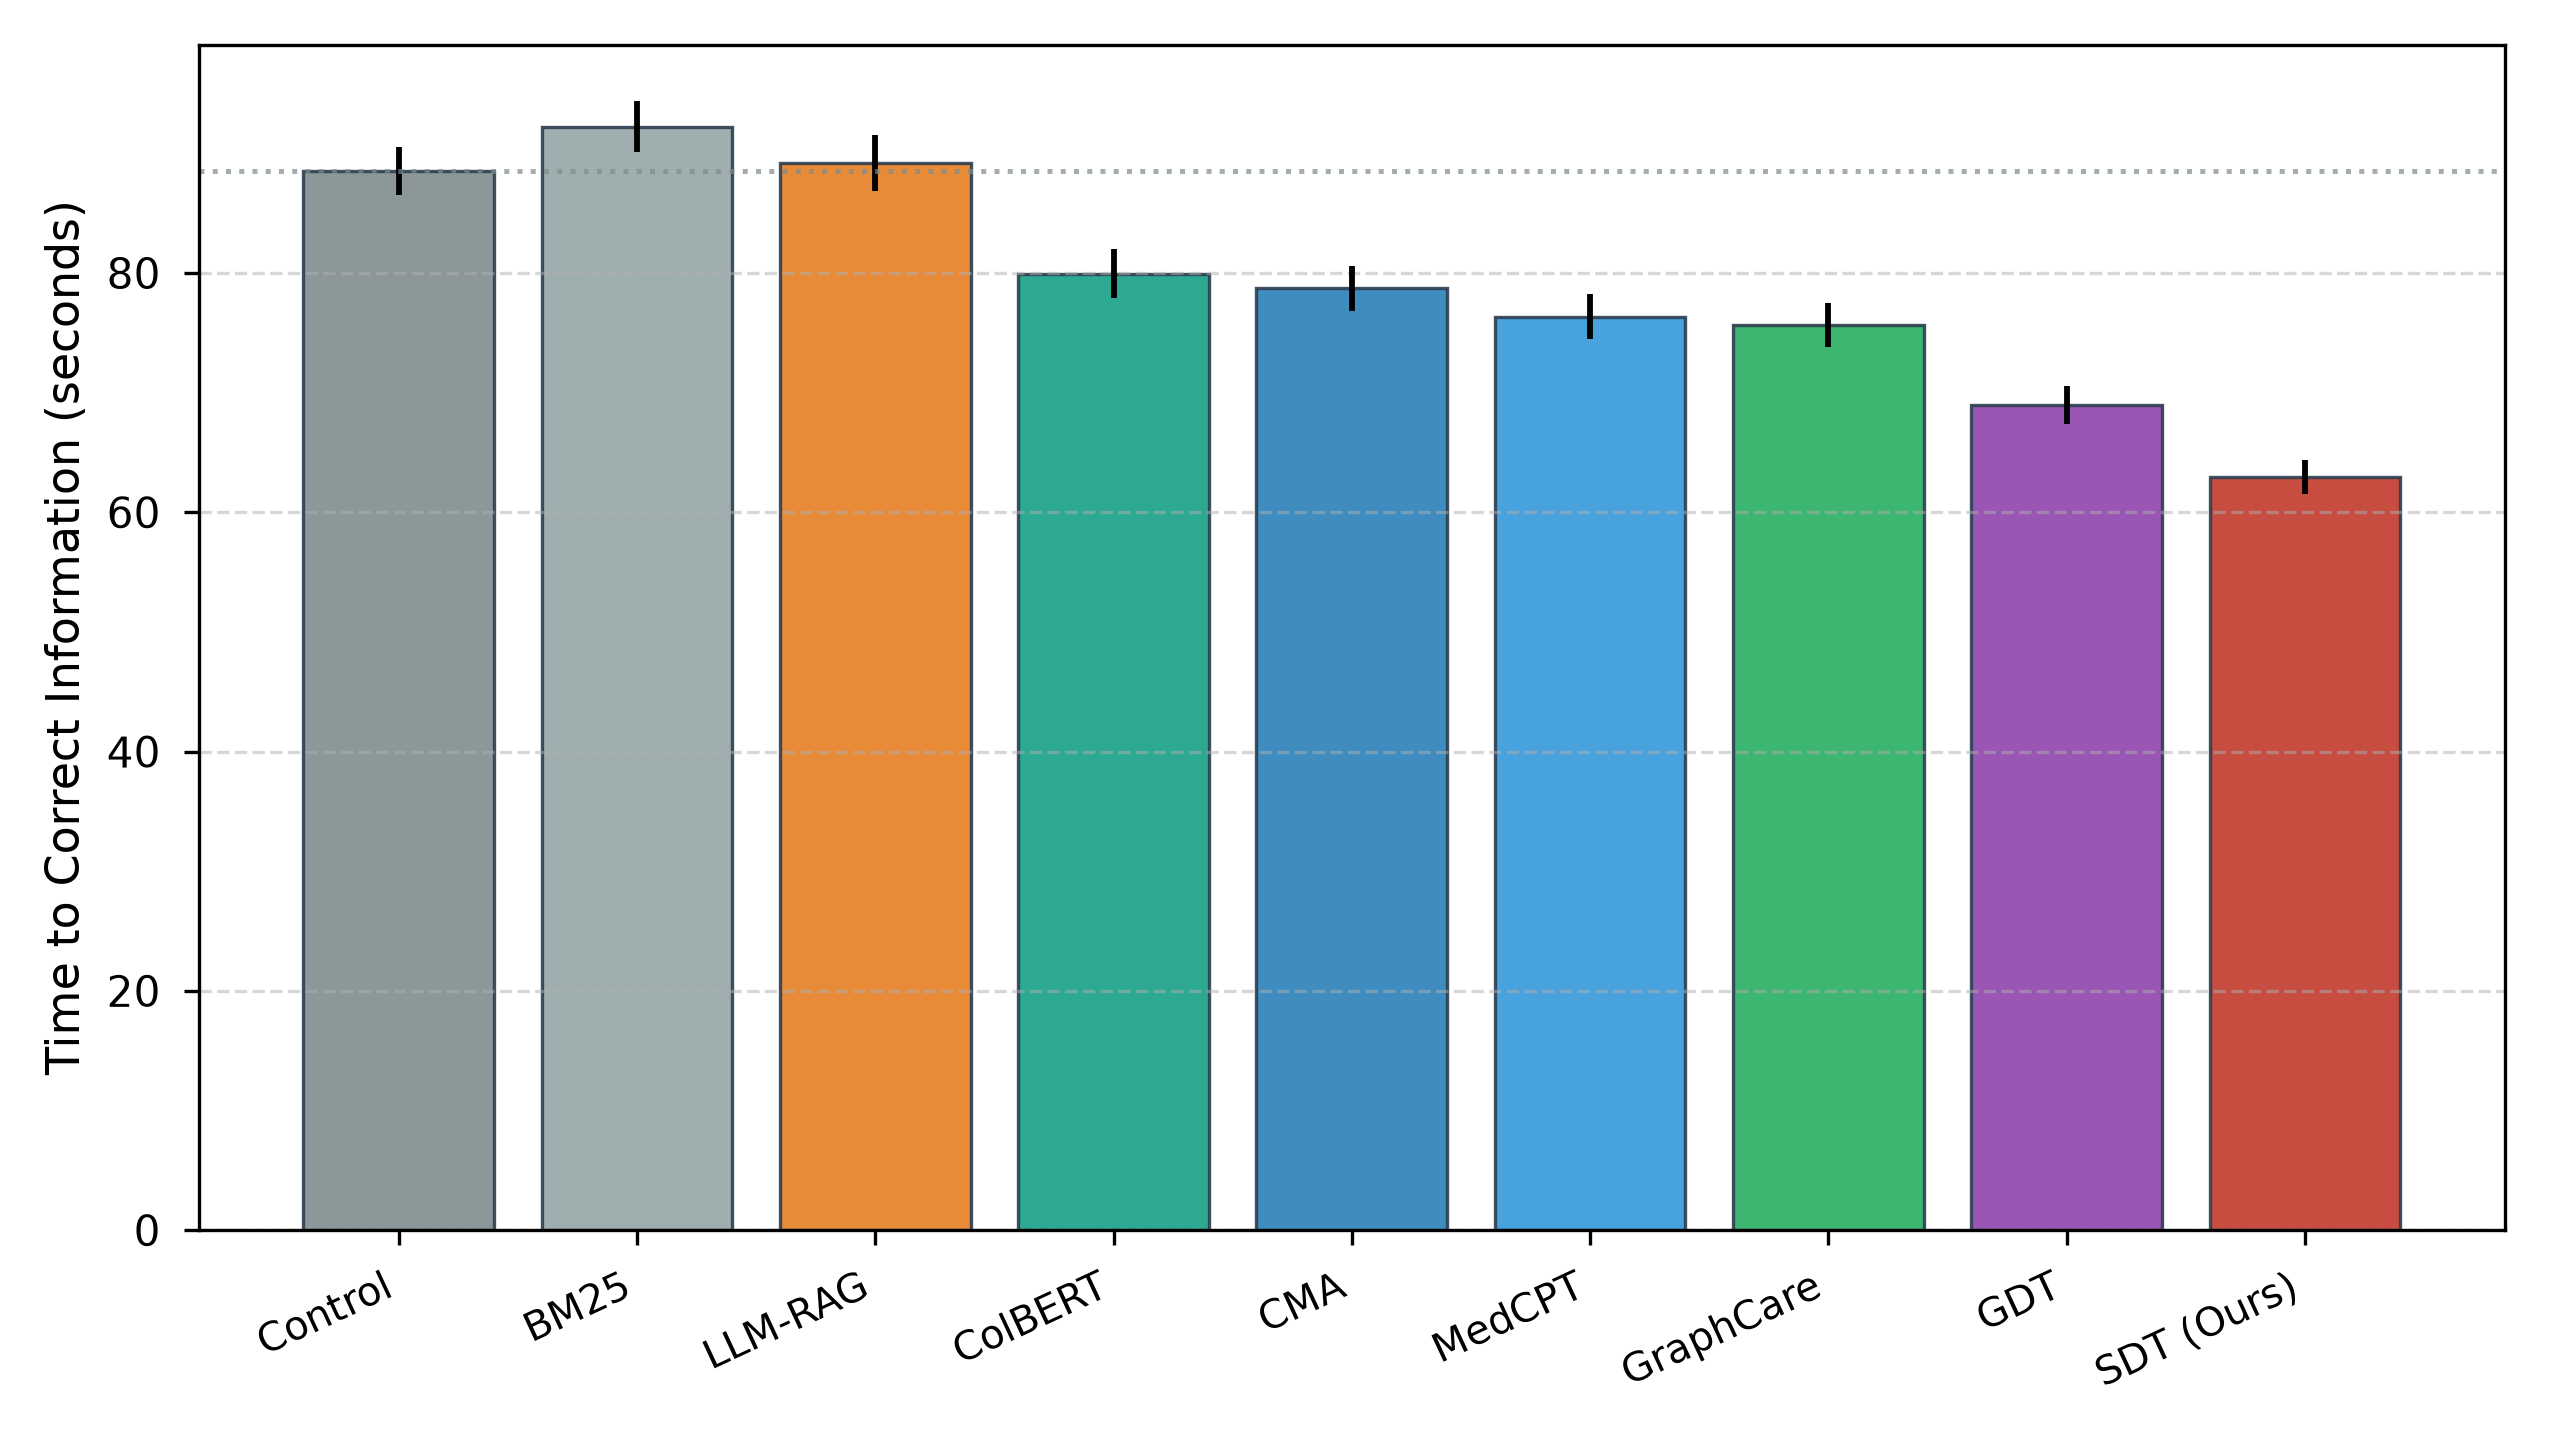
\includegraphics[width=0.85\textwidth]{fig_ttci_bar.png}
  \caption{Mean Time-to-Correct-Information (TTCI) across 9 experimental conditions.}
  \label{fig:ttci_bar}
\end{figure}

\begin{figure}[h!]
  \centering
  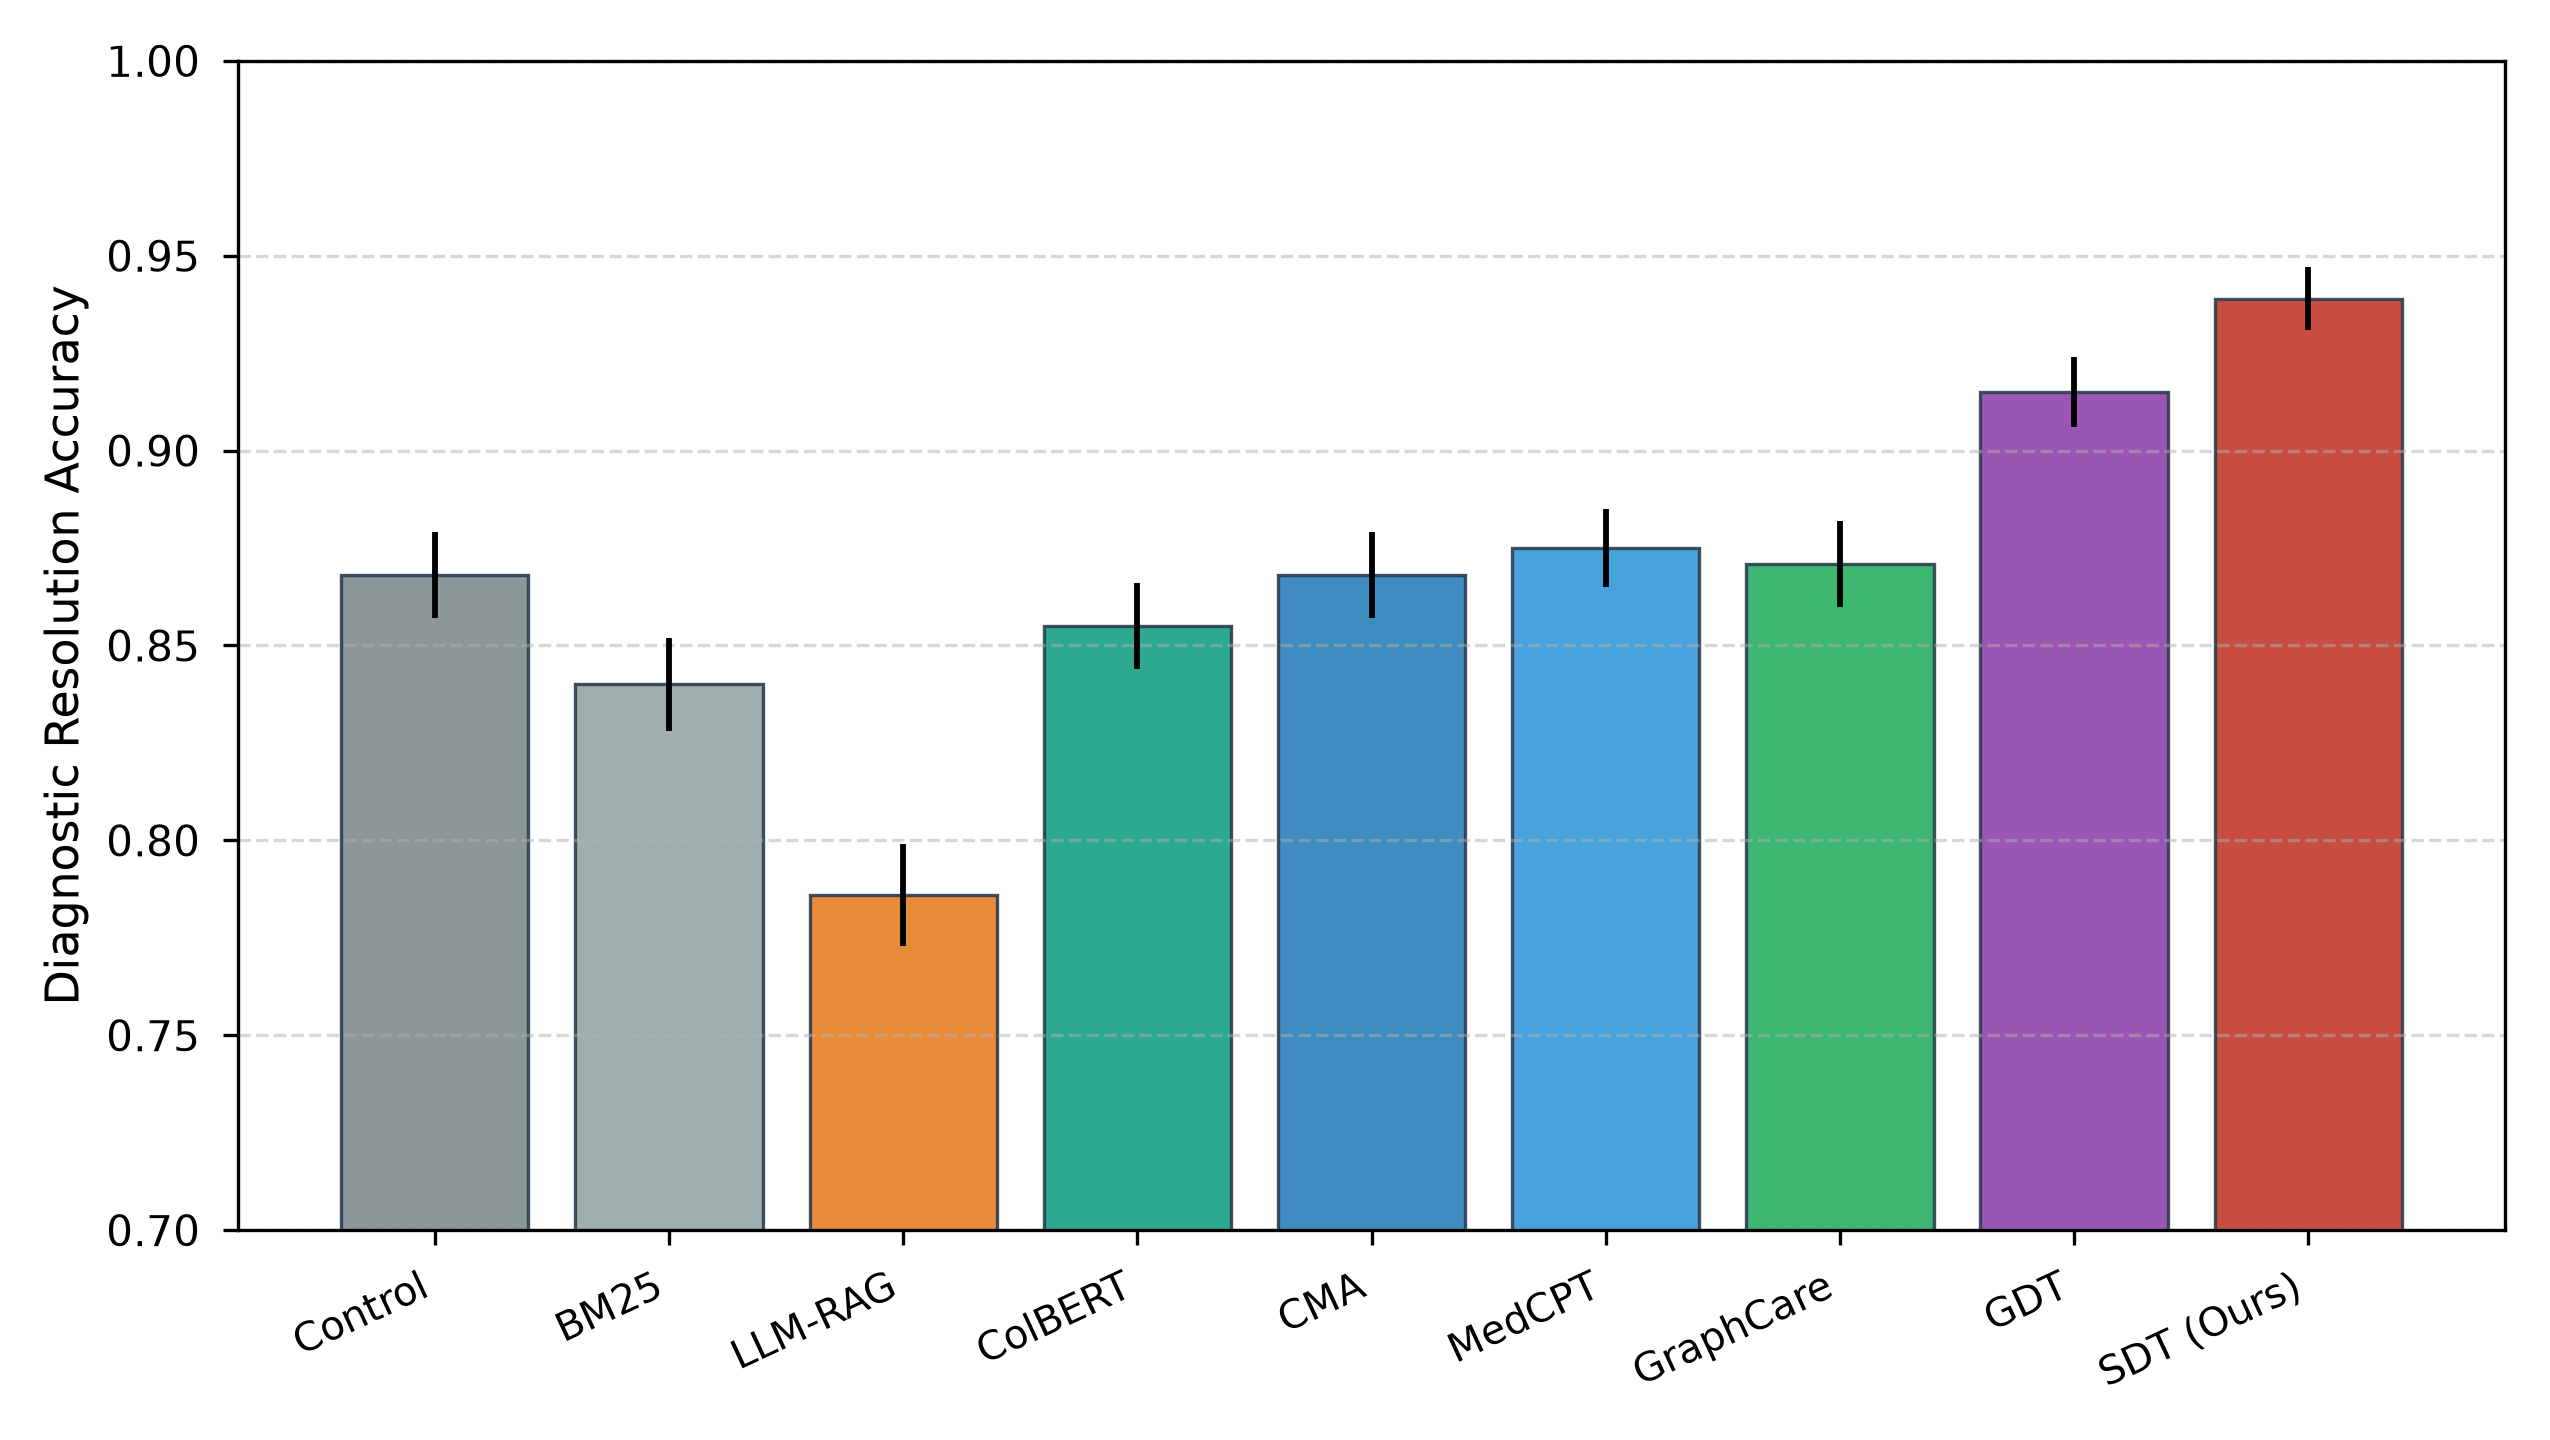
\includegraphics[width=0.85\textwidth]{fig_accuracy_bar.png}
  \caption{Diagnostic retrieval accuracy across conditions.}
  \label{fig:acc_bar}
\end{figure}

\begin{figure}[h!]
  \centering
  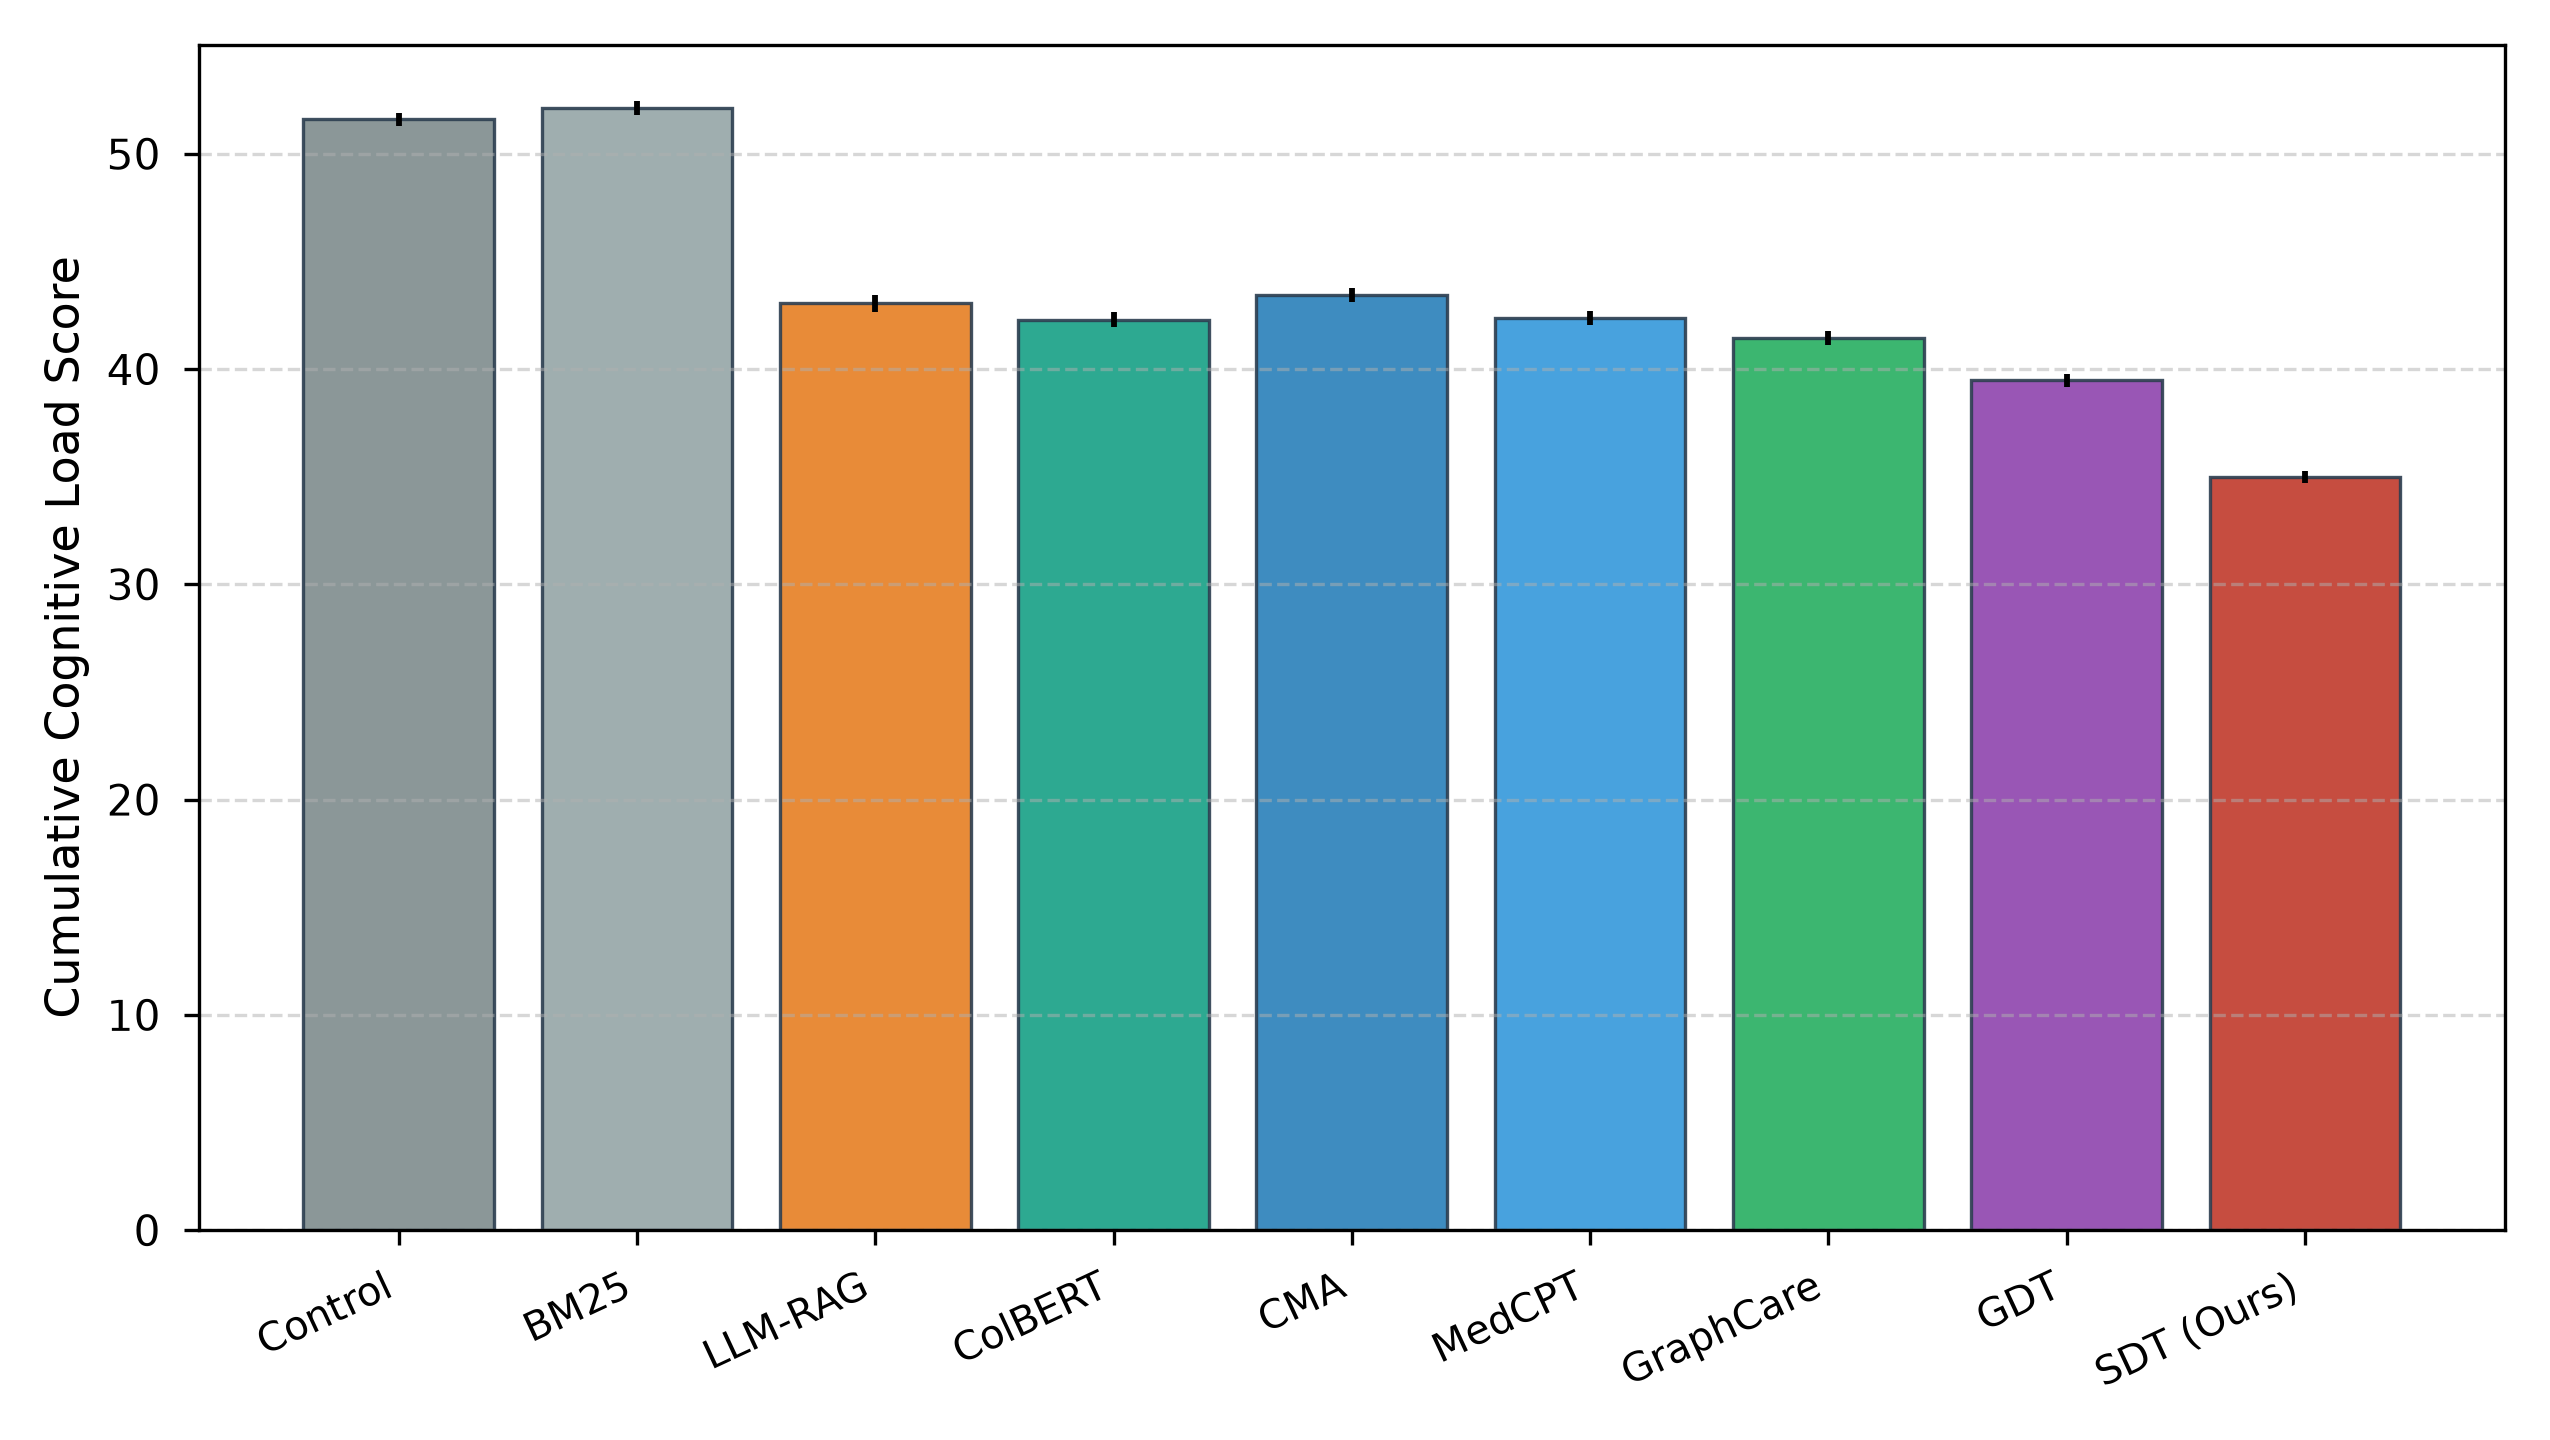
\includegraphics[width=0.85\textwidth]{fig_cognitive_load_bar.png}
  \caption{Modeled cognitive load across conditions.}
  \label{fig:cog_bar}
\end{figure}

\begin{figure}[h!]
  \centering
  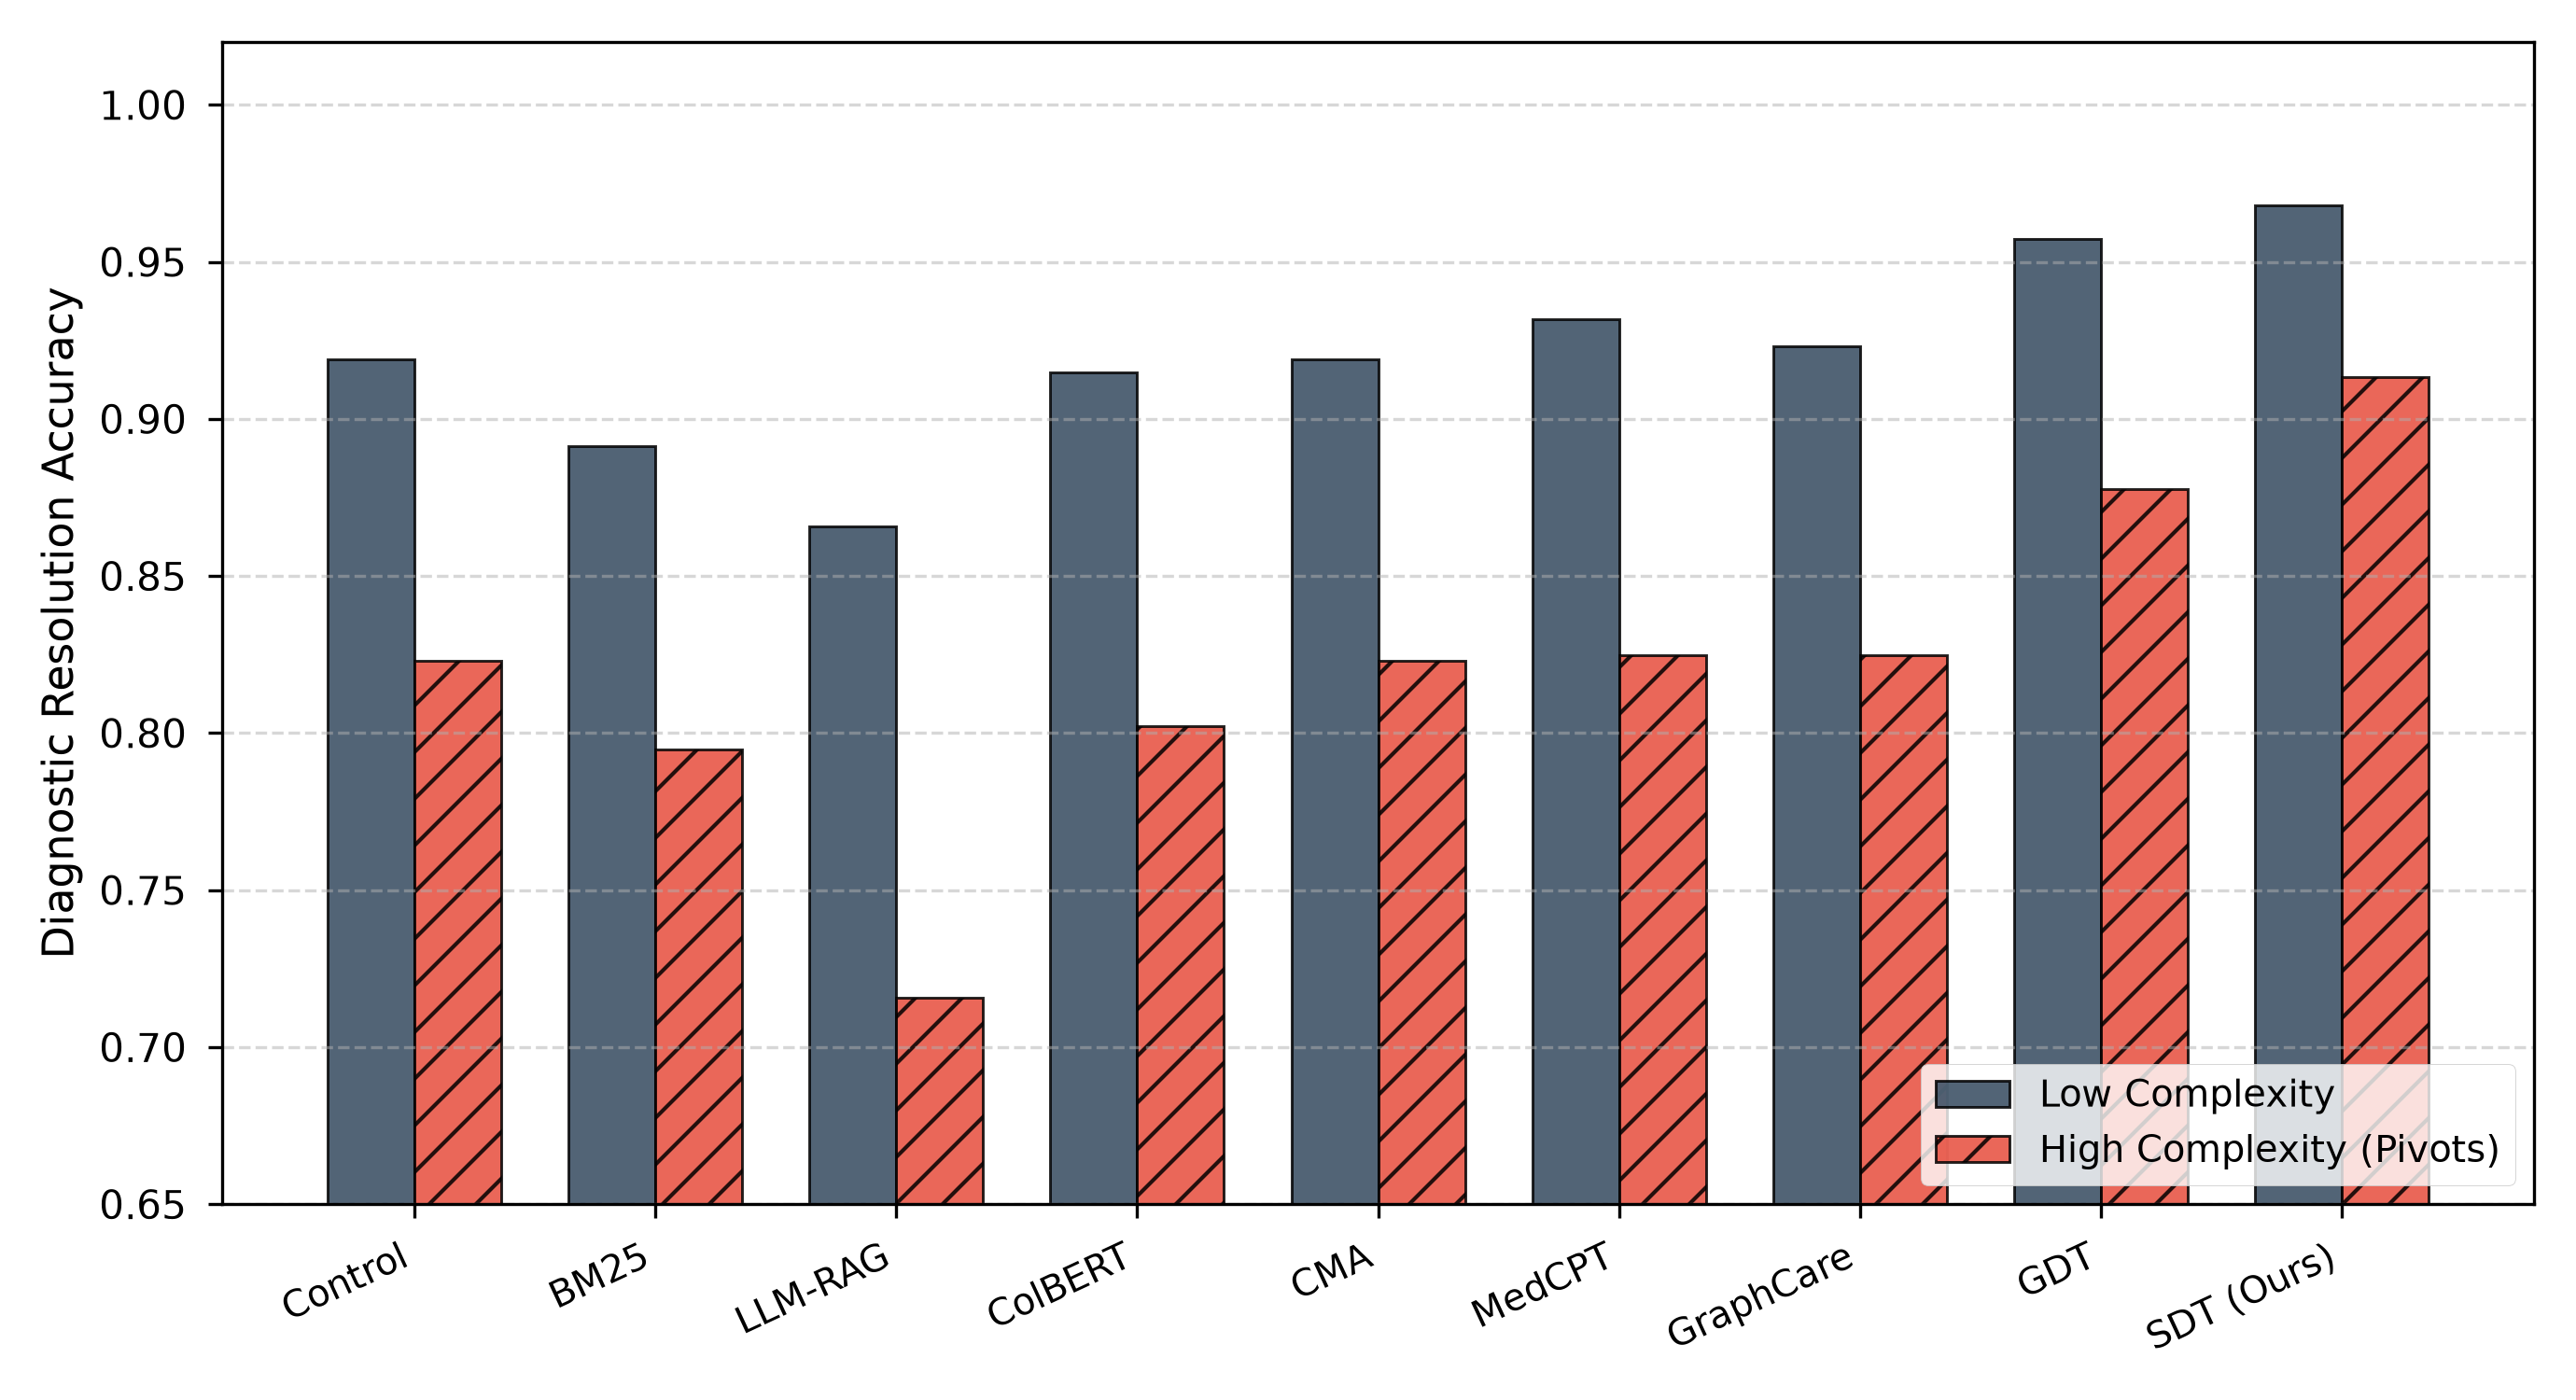
\includegraphics[width=0.85\textwidth]{fig_subgroup_accuracy.png}
  \caption{Diagnostic accuracy stratified by case complexity.}
  \label{fig:subgroup_acc}
\end{figure}

\begin{figure}[h!]
  \centering
  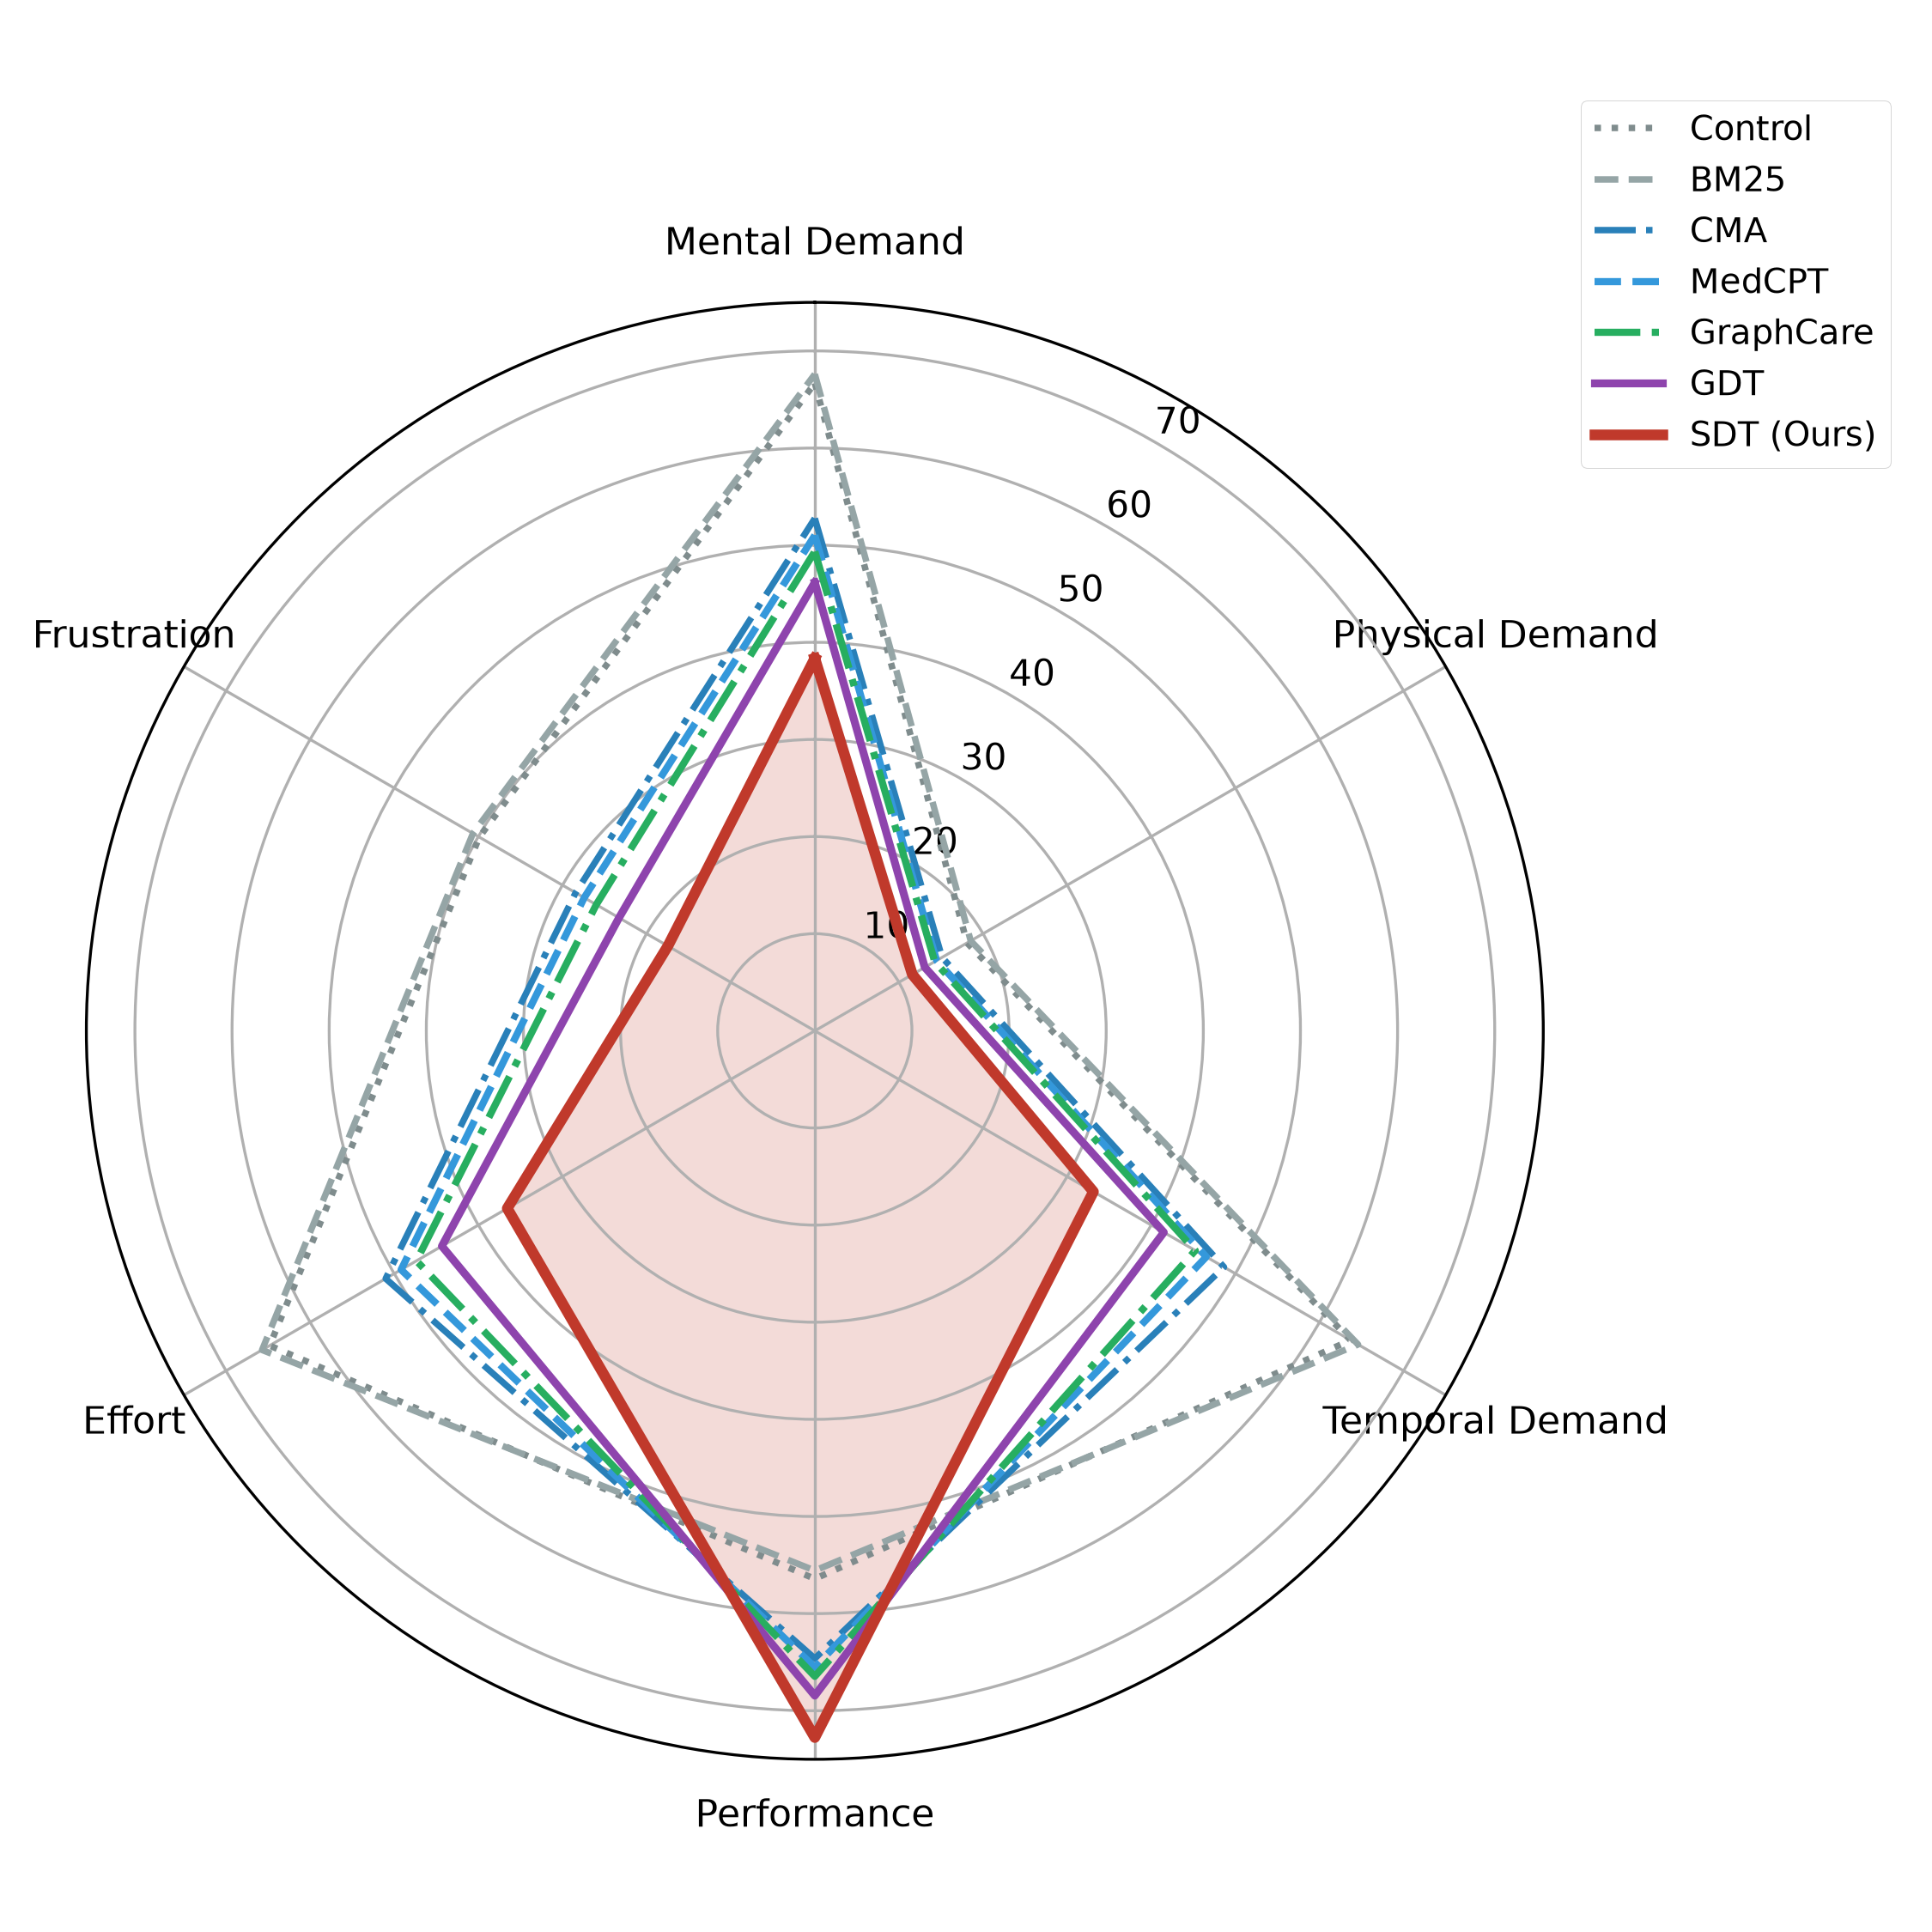
\includegraphics[width=0.85\textwidth]{fig_nasa_tlx_radar.png}
  \caption{Multi-dimensional NASA-TLX subjective workload profile.}
  \label{fig:tlx_radar}
\end{figure}

\begin{figure}[h!]
  \centering
  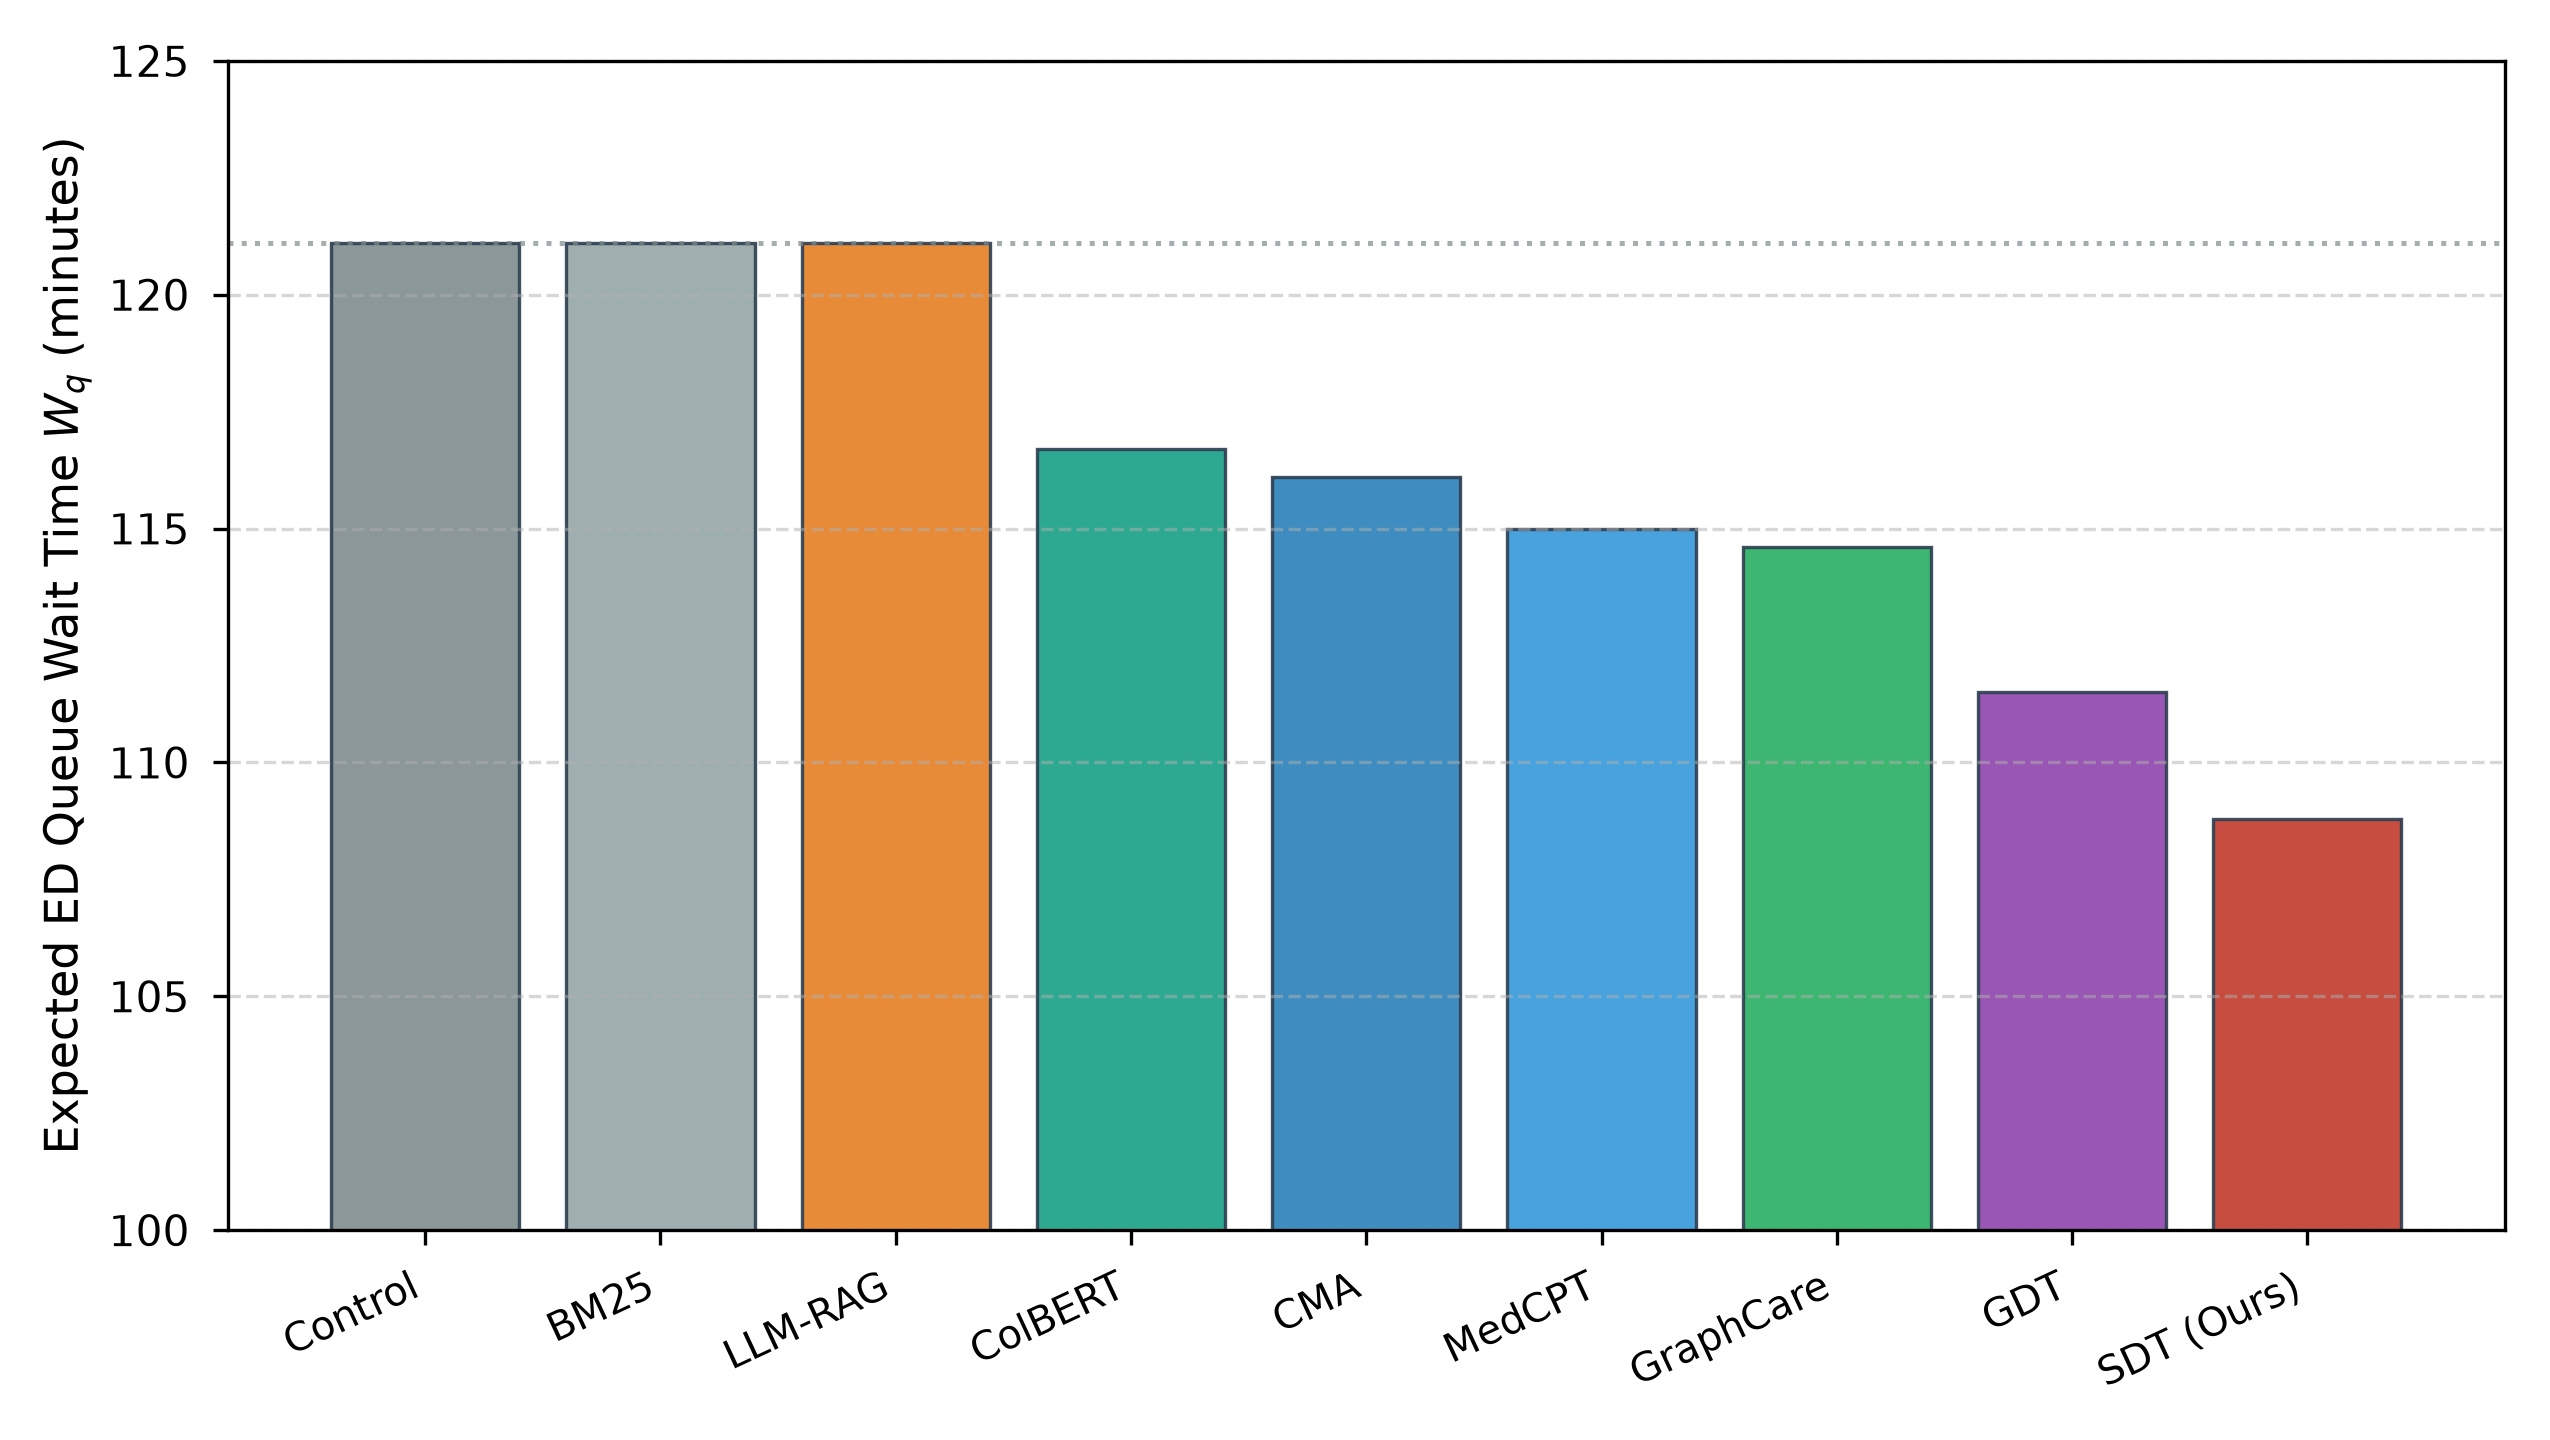
\includegraphics[width=0.85\textwidth]{fig_queueing_impact.png}
  \caption{Emergency Department operational queue waiting time ($W_q$).}
  \label{fig:queueing_impact}
\end{figure}

\end{document}
